% latex4wp.tex		-*- LaTeX -*-
%
% LaTeX per utenti di word processor
% di Guido Gonzato, guido.gonzato (at) gmail.com
%
% Questo documento \`e stato scritto con l'editor Jed,
% http://www.jedsoft.org/jed, e il mio nuovo LaTeX mode
% disponibile presro i mirror CTAN mirrors,
% http://www.ctan.org/tex-archive/support/jed
%
% Ultimo aggiornamento: 8 Gennaio 2015

% debug
% \overfullrule=15pt

% TO DO: rivedere tutti i \medskip e \bigskip, forse vanno tolti

\documentclass[a4paper,11pt]{article}
\usepackage[margin=2.5cm]{geometry}
\usepackage[italian]{babel} % lingua italiana
\usepackage{color}          % colori
\usepackage{ifpdf}
\ifpdf
  \usepackage[pdftex]{graphicx}
  \pdfcompresslevel=9
\else
  \usepackage{graphicx}
\fi
\usepackage{alltt}     % come verbatim, ma onora i comandi LaTeX
\usepackage{dcolumn}   % allinea i numeri
\usepackage{url}       % url e link
\usepackage{colortbl}  % tabelle a colori
\usepackage{pifont}    % dinglist
\usepackage{fancyvrb}  % verbatim con variazioni
\usepackage{boxedminipage} % minipage col bordo
\usepackage{framed}    % bordi intorno a oggetti
\usepackage{rotating}  % ruota oggetti
\usepackage[colorlinks,
            urlcolor=blue,
	    filecolor=magenta,
	    linkcolor=darkred,
	    hyperfootnotes=false]{hyperref} % link navigabili
\usepackage{fancyhdr}  % intestazioni e pie' di pagina
\usepackage{marvosym}  % Euro e altri caratteri
\usepackage[gen]{eurosym} % Euro
\usepackage{mflogo}    % logo Metafont
\usepackage{setspace}  % spaziatura personalizzata
\usepackage{tabularx}  % ambiente tabular esteso
\usepackage{exa}       % per comporre esempi (pacchetto locale)
\usepackage{enumerate} % arg. opzionali per enumerate
\usepackage{wrapfig}   % testo che scorre intorno a figure
\usepackage[normalem]{ulem} % sottolineature
\usepackage{slashbox}  % caselle barrate in tabelle
\usepackage{paralist}  % elenchi nei paragrafi
\usepackage[version=3]{mhchem} % formule chimiche
\usepackage{lettrine}  % lettere grandi a inizio paragrafo

\urlstyle{same} % url con font normale

% --- Definizioni e nuovi comandi ---

\def\version {1.0.8}
\def\bs      {\textbackslash}
\def\unix    {\textsc{Unix}}
% \def\warning {\marginpar{\Huge{\textcolor{red}{\Stopsign}}}}
\def\note    {\marginpar{\Huge{\textcolor{magenta}{\Writinghand}}}}
\def\PS      {\textsc{PostScript}}
\definecolor {darkred}{rgb}{0.75,0,0}

\newcounter{fnsym}
\setcounter{fnsym}{1}
%\newcounter{tmpbaselineskip}
%\setlength{tmpbaselineskip}{\value{\baselineskip}}

% perch\'e non mi considera le regole?
\hyphenation{in-te-sta-zio-ne u-sa-no}

\newenvironment{margini}[2]
{ 
  \begin{list}{} {
    \setlength{\leftmargin}{#1}
    \setlength{\rightmargin}{#2}
  } \item }
{\end{list}}

\newenvironment{warn}
{ % beg def
  \medskip
  \begin{minipage}[t]{0.1\linewidth}
    \vspace{0pt}
    \textcolor{magenta}{\Huge{\Pointinghand}}
  \end{minipage}%
  \begin{minipage}[t]{0.88\textwidth}
    \vspace{0pt}
    \begin{small}
      \begin{spacing}{0.97}
}
{ % end def
      \end{spacing}
    \end{small}
  \end{minipage}
  \medskip
}

\newcommand{\package}[1]
{\textsf{#1}}

\newcommand{\parm}[1]
{\texttt{#1}}

\newcommand{\cmdparm}[1]
{\textsl{#1}}

\newcommand{\env}[1]
{\texttt{#1}}

\newcommand{\cmd}[1]
{\texttt{\bs{}#1}}

\newcommand{\cmdline}[1]
{\texttt{#1}}

\newcommand{\menu}[1]
{\textsf{#1}}

\newcommand{\entry}[2]
{\textsf{#1/#2}}

\newcommand{\app}[1]
{\textsf{#1}}

\newcommand{\file}[1]
{\texttt{#1}}

\newcommand{\style}[1]
{\texttt{#1}}

\newcommand{\ltx}[1]
{\texttt{#1}}

\newcommand{\car}[1]
{\texttt{#1}}

% --- fine delle definizioni ---

% si va in scena

\begin{document}

\frenchspacing % spazio dopo i punti sempre uguale
\pagenumbering{roman}
\setlength{\parindent}{0pt}
\setlength{\parskip}{3pt}

\title{\LaTeX{} per utenti di word processor\\versione \version}

\author{Guido Gonzato, PhD --
\texttt{guido.gonzato@gmail.com}}

\date{\today}

\maketitle

\begin{abstract}

  La composizione di testi con \LaTeX{} offre numerosi vantaggi
  rispetto alla videoscrittura. Tuttavia, gli utenti di word processor
  che passano a \LaTeX{} solitamente incontrano alcune difficolt\`a
  nell'ottenere gli stessi risultati con questo nuovo strumento.
  Questo manuale intende facilitare la transizione tracciando dei
  confronti tra videoscrittura e composizione con \LaTeX. Vengono
  elencate le principali azioni di un word processor e gli equivalenti
  comandi in \LaTeX, con numerosi esempi.

\end{abstract}

\begin{footnotesize}
  \tableofcontents
  \listoftables
  \listoffigures
\end{footnotesize}

% INTRODUCTION

\pagestyle{fancy}
\pagenumbering{arabic}

\section{Introduzione}

Vorrei iniziare precisando che questo documento \emph{non \`e} una
guida introduttiva a \LaTeX! Do per scontato che il lettore possegga
le necessarie conoscenze di base a proposito di \LaTeX{} e dei suoi
comandi. Lo scopo di questa guida \`e mostrare come sostituire un word
processor utilizzando \LaTeX{} al suo posto.

I word processor sono la principale applicazione dell'ufficio moderno.
Vengono percepiti come facili da usare, e di solito una segretaria
impara ad usarli in tempi ragionevolmente brevi. Il problema di questi
programmi \`e che, di versione in versione, diventano sempre pi\`u
lenti, ingombranti\footnote{tanto tempo fa, scrissi la mia tesi di
laurea su un home computer da 128K di RAM, basato su Z80. Il word
processor WordStar e la mia tesi stavano comodi su un floppy avviabile
CP/M da 720K, e avanzava un sacco di spazio!}, pieni di bug, inclini a
bloccarsi, costosi, attaccabili da virus e incompatibili tra loro. Per
non parlare della qualit\`a del loro output.

\LaTeX{} \`e una buona alternativa; ma per chi \`e abituato a pensare
in termini di videoscrittura, pu\`o rivelarsi poco intuitivo. In altre
parole, si potrebbero volere le caratteristiche di un word
processor{\ldots} con \LaTeX. Sarebbe una buona cosa sapere come
ottenere con \LaTeX{} i risultati che si sa come ottenere col proprio
word processor di riferimento.

Ecco perch\'e ho scritto questa guida rapida. Come ho gi\`a detto, si
assume che il lettore abbia minime conoscenze di \LaTeX; se non fosse
cos\`\i{}, raccomando di visitare il sito
\url{http://www.ctan.org/starter.html} e scaricare, in traduzione
italiana, ``The (Not So) Short Introduction to \LaTeX2e''. Un'altra
ottima guida per iniziare (solo in inglese, purtroppo) \`e
\url{http://en.wikibooks.org/wiki/LaTeX/}.

Nelle prossime sezioni esamineremo i menu di un word processor
immaginario, mostrando le corrispondenti azioni in \LaTeX{} per
ottenere lo stesso risultato.

% -----

\subsection{Informazioni preliminari}

Molte funzionalit\`a del word processor sono implementate dall'editor
con cui si scrive; altre da comandi \LaTeX{} standard; altre ancora si
ottengono utilizzando dei pacchetti (\emph{package}) \LaTeX. Si tratta
di insiemi di macro che estendono \LaTeX{} con nuovi comandi ed
ambienti (\emph{environment}). Sono disponibili centinaia di
pacchetti: si tratta di sapere dove trovarli, capire quale pacchetto
fa che cosa e come installarli. Ulteriori informazioni sui pacchetti
sono disponibili alla Sezione~\ref{sec:packages}.

I pacchetti e altro materiale correlato sono disponibili presso i siti
che costituiscono il CTAN: Comprehensive TeX Archive Network. Ho gi\`a
citato il sito \url{http://www.ctan.org}, che ha numerosi mirror.
D'ora in poi, con \href{http://www.ctan.org}{CTAN:} si intende: ``il
vostro mirror CTAN di riferimento, a partire dalla directory
\path{TeX}''. Ad esempio, si pu\`o scaricare \LaTeX{} per il proprio
sistema operativo dal sito
\href{http://ftp.uniroma2.it/TeX/systems/}{CTAN://systems}, cio\`e
\url{http://ftp.uniroma2.it/TeX/systems/}.

Per scrivere i documenti \`e necessario un buon editor di testi. Per
chi inizia, \`e raccomandabile una \emph{shell \LaTeX}, ovvero un
editor dedicato alla scrittura di sorgenti in \LaTeX, con anteprima e
altre funzionalit\`a. Suggerisco di provare uno dei programmi elencati
di seguito; sono tutti software Free/O\-pen Source.

\begin{itemize}

  \item Texmaker (multipiattaforma):\\
  \url{http://www.xm1math.net/texmaker/index.html}

 \item TeXstudio (multipiattaforma):\\
  \url{http://texstudio.sourceforge.net/}

  \item TeXworks (multipiattaforma):\\
  \url{http://tug.org/texworks/}
  
%  \item LyX, una shell quasi WYSIWYG (multipiattaforma):\\
%  \url{http://www.lyx.org/}
  
  \item TeXShop (Mac OS X):\\
  \url{http://www.uoregon.edu/~koch/texshop/}
  
  \item TeXnicCenter (Windows):\\
  \url{http://www.texniccenter.org/}
    
\end{itemize}

Informazioni su \LaTeX{} in ambiente Macintosh si trovano
all'indirizzo \url{http://www.esm.psu.edu/mac-tex/}.

% -----

% EDITOR-SUPPORTED

\subsubsection{Caratteristiche fornite dall'editor}

\LaTeX{} \`e ``solo'' un programma di impaginazione: azioni come il
copia e incolla, cerca e sostituisci ecc. sono compito dell'editor.
La Tabella~\ref{tab:editing} riassume i principali comandi di alcuni
editor per utenti esperti: GNU \app{emacs} e \app{vim}, pi\`u 
\app{jed} configurato per le combinazioni di tasti WordStar/Borland
IDE.

\begin{table}[htbp]
\begin{center}
\begin{tabular}{lccc} \hline
\textbf{Azione} & \textbf{Emacs} & \textbf{Vim} & \textbf{Jed} \\
\hline
modalit\`a comando & \texttt{Alt-X} & \texttt{ESC} & \texttt{Alt-X} \\
modalit\`a inserimento & n/a & \texttt{i a o O} & n/a \\
modalit\`a line editor & n/a & \texttt{:} & n/a \\
%\hline
\multicolumn{4}{c}{\textbf{\rule{0pt}{0.5cm}operazioni sui file}}\\[0.3cm]
%\hline
apri file & \texttt{Ctrl-X Ctrl-F} & \texttt{:e} & \texttt{Ctrl-KE}\\
inserisci file & \texttt{Ctrl-Xi} & \texttt{:r} & \texttt{Ctrl-KR}\\
salva file & \texttt{Ctrl-X Ctrl-S} & \texttt{:w} & \texttt{Ctrl-KD}\\
salva come & \texttt{Ctrl-X Ctrl-W name} & \texttt{:w name} & \texttt{Ctrl-KS}\\
chiudi file & \texttt{Ctrl-XK} & \texttt{:q} & \texttt{Ctrl-KQ}\\
cambia buffer & \texttt{Ctrl-XB} & \texttt{bN} & \texttt{Ctrl-KN}\\
undo & \texttt{Ctrl-XU} & \texttt{u} & \texttt{Ctrl-U}\\
redo & \texttt{Ctrl-\^} & \texttt{Ctrl-R} & \texttt{Ctrl-G Ctrl-U}\\
esci & \texttt{Ctrl-X Ctrl-C} & \texttt{:qa!} & \texttt{Ctrl-KX}\\
%\hline
\multicolumn{4}{c}{\textbf{\rule{0pt}{0.5cm}spostamento}}\\[0.3cm]
%\hline
parola a sx & \texttt{Alt-B} & \texttt{b} & \texttt{Ctrl-A}\\
parola a dx & \texttt{Alt-F} & \texttt{w} & \texttt{Ctrl-F}\\
inizio linea & \texttt{Ctrl-A} & \texttt{0} & \texttt{Ctrl-QS}\\
fine linea & \texttt{Ctrl-E} & \texttt{\$} & \texttt{Ctrl-QD}\\
pagina su & \texttt{Alt-V} & \texttt{Ctrl-U} & \texttt{Ctrl-R}\\
pagina gi\`u & \texttt{Ctrl-V} & \texttt{Ctrl-D} & \texttt{Ctrl-C}\\
inizio buffer & \texttt{Alt-<} & \texttt{1G} & \texttt{Ctrl-QR}\\
fine buffer & \texttt{Alt->} & \texttt{G} & \texttt{Ctrl-QC}\\
linea n. & \texttt{Alt-G n.} & \texttt{n.G} & \texttt{Ctrl-QI}\\
%\hline
\multicolumn{4}{c}{\textbf{\rule{0pt}{0.5cm}cancellazione}}\\[0.3cm]
%\hline
carattere a sx & \texttt{Ctrl-H} & \texttt{X} & \texttt{BS}\\
carattere a dx & \texttt{Ctrl-D} & \texttt{x} & \texttt{Alt-G}\\
parola a sx & \texttt{Alt-DEL} & \texttt{db} & \texttt{Alt-BS}\\
parola a dx & \texttt{Alt-D} & \texttt{dw} &\texttt{Ctrl-T} \\
fine linea & \texttt{Ctrl-K} & \texttt{d\$} & \texttt{Ctrl-QY} \\
linea & \texttt{Ctrl-A Ctrl-K} & \texttt{dd} & \texttt{Ctrl-Y} \\
%\hline
\multicolumn{4}{c}{\textbf{\rule{0pt}{0.5cm}cerca \& sostituisci}}\\[0.3cm]
%\hline
cerca & \texttt{Ctrl-S text} & \texttt{/text} & \texttt{Ctrl-QS}\\
sostituisci & \texttt{Alt-\%} & \texttt{:s/old/new/g} & \texttt{Ctrl-QA}\\
%\hline
\multicolumn{4}{c}{\textbf{\rule{0pt}{0.5cm}blocchi}}\\[0.3cm]
%\hline
inizia blocco & \texttt{Ctrl-SPACE} & \texttt{v} & \texttt{Ctrl-KB} \\
taglia & \texttt{Ctrl-W} & \texttt{D} & \texttt{Ctrl-KY} \\
copia & \texttt{Alt-W} & \texttt{Y} & \texttt{Ctrl-KH} \\
incolla & \texttt{Ctrl-Y} & \texttt{P} & \texttt{Ctrl-KC} \\
\hline
\end{tabular}
\caption{Combinazioni di tasti per Emacs, Vim e Jed in modalit\`a IDE.}
\label{tab:editing}
\end{center}
\end{table}

% -----

% ADDING PACKAGES

\subsubsection{Come aggiungere pacchetti}
\label{sec:packages}

Le informazioni che seguono valgono per \app{TeX Live}, fornito con le
principali distribuzioni GNU/Linux; potrebbero funzionare anche con
\app{MacTeX}, ma non ne ho diretta esperienza. Le istruzioni per
\app{MiKTeX} (probabilmente l'implementazione pi\`u diffusa in
ambiente Windows) verranno date pi\`u avanti.

Un numero elevato di pacchetti viene di norma fornito con la
distribuzione GNU/Linux; ad esempio, Ubuntu ha molti pacchetti
\file{.deb} del tipo \app{texlive-*}. Attenzione all'ambiguit\`a del
termine: si parla di \emph{pacchetti} \file{.deb} che contengono
\emph{pacchetti} \LaTeX.

Se si deve installare un pacchetto che non viene fornito in formato
\file{.deb}, si seguano queste istruzioni.

\begin{enumerate}

  \item creare questo albero di directory:
  
  \begin{verbatim}
  $ mkdir -p ~/texmf/tex/latex
  \end{verbatim}
  
  I nuovi pacchetti saranno installati a partire da questa directory.

  \item scaricare il pacchetto dal mirror CTAN preferito (di solito
  come archivio zip); supponiamo si chiami \app{pippo.zip}
  
  \item decomprimerlo nella directory giusta:
  
  \begin{verbatim}
  $ mkdir ~/texmf/tex/latex/pippo
  $ mv pippo.zip ~/texmf/tex/latex/pippo
  $ cd ~/texmf/tex/latex/pippo ; unzip pippo.zip
  \end{verbatim}
 
  \item se non \`e presente un file \file{.sty}, eseguire il comando
  \cmdline{latex pippo.ins} o \cmdline{latex pippo.dtx} per crearlo;
  
  \item eseguire il comando \cmdline{texhash \~{}/texmf}.
    
\end{enumerate}

Per aggiungere un pacchetto a \app{MiKTeX}, creare la directory
\path{latex\pippo} al di sotto di \path{C:\localtexmf\tex\} e copiarvi
i file del pacchetto \app{pippo.zip}. Procedere come mostrato per
\app{TeX Live}, quindi eseguire \app{MiKTeX Options} e fare clic su
``Refresh now''. Oppure, da linea di comando scrivere 
\cmdline{initexmf -u}.

Una volta che il pacchetto \`e installato, per utilizzarlo nei propri
documenti si aggiunge una linea sotto la dichiarazione
\ltx{documentclass}:

\begin{verbatim}
\usepackage{pippo}
\end{verbatim}

% -----

\subsubsection{Aggiungere la pagina Info}
\label{sec:infopage}

Le pagine `Man' e `Info', accessibili da shell in ambiente \unix{} e
Linux, forniscono documentazione per molti pacchetti software. Se
nella vostra distribuzione \LaTeX{} manca il file \file{latex2e.info},
fate cos\`\i{}:

\begin{enumerate}
  
  \item scaricatela da 
  \url{http://tug.ctan.org/info/latex2e-help-texinfo/latex2e.info};
  
  \item eseguite questi comandi:
  
  \begin{verbatim}
  $ sudo cp latex2e.info /usr/share/info/
  $ sudo ginstall-info latex2e.info dir
  \end{verbatim}
   
\end{enumerate}

Ora il comando \cmdline{info latex} o \cmdline{info latex2e} \`e
disponibile.

% -----


% GOLDEN RULES

\subsection{Le ``regole d'oro''}

Prima di iniziare, vorrei sottolineare quanto segue:

\begin{enumerate}

  \item \`e necessario abituarsi a \emph{dare una struttura} ai propri
  documenti: bisogna pensare in termini di parti, capitoli, sezioni e
  cos\`\i{} via. Questo vale anche se non si sta scrivendo un articolo
  scientifico.
  
  \item \label{rule:mess} \LaTeX{} scoraggia esplicitamente l'utente
  dal pasticciare con i parametri di formattazione. Non ci si deve
  preoccupare troppo dell'\emph{aspetto} di quello che si sta
  scrivendo, quanto piuttosto del \emph{contenuto}.

\end{enumerate}

Applicando queste semplici regole di base, i documenti assumeranno
magicamente un look professionale.

Detto questo, questa guida (che un po' contravviene alla seconda
regola!) aiuter\`a a superare quanto dettato dalla regola d'oro
n.~\ref{rule:mess}. In questo modo, oltre a documenti ben strutturati
si potr\`a scrivere materiale come volantini, avvisi, poster, {\ldots}

\bigskip

{\color{blue} \dingline{45}}

% -----

% FILE

\section{Il menu \menu{File}}

Ovviamente, alcune voci di menu non hanno nulla a che vedere con \LaTeX{}:
\entry{File}{Apri}, \entry{File}{Salva}, \entry{File}{Chiudi}
dipendono dall'editor.

% -----

% FILE/NEW

\subsection{\entry{File}{Nuovo}}
\label{sec:filenew}

Questo \`e l'equivalente \LaTeX{} di una pagina vuota:

\begin{Verbatim}[fontsize=\small]
\documentclass{article}
\thispagestyle{empty} % niente numero di pagina
\begin{document}
% Questo \`e un commento. Qui sotto c'e' una riga vuota.

\end{document}
\end{Verbatim}

Poich\'e i documenti scritti in \LaTeX{} sono solitamente forniti di
una struttura, l'esempio che segue \`e pi\`u realistico:

\begin{Verbatim}[fontsize=\small]
\documentclass[a4paper,12pt]{article}
\begin{document}
\title{Il mio documento}
\author{Mario Rossi}
\date{Roma, \today}
\maketitle
\begin{abstract}
Questo \`e un brevissimo articolo.
\end{abstract}
\tableofcontents
\listoftables
\listoffigures
\section{Prima sezione}
\label{sec:start}
Questo \`e il testo della sezione. Si veda \cite{Gonzato} per
ulteriori dettagli.
\section{End}
\label{sec:end}
Questa \`e la fine del documento. Si veda la Sezione~\ref{sec:start}
per rileggerlo.
\begin{thebibliography}{99}
\bibitem{Gonzato} Gonzato G. \textit{\LaTeX{} for Word Processor
Users}. CTAN, 2001-2015.
\end{thebibliography}
\end{document}
\end{Verbatim}

Altri modelli di documento verranno mostrati
all'Appendice~\ref{ap:templates}.

% -----

% FILE/SAVE AS

\subsection{\entry{File}{Salva con nome{\ldots}}}

I programmi che seguono sono utili per convertire un documento scritto
in \LaTeX{} in altri formati:

\begin{itemize}

  \item \app{\TeX4ht} \`e probabilmente il migliore convertitore da
  \LaTeX{} ad HTML:\\
  \url{http://www.cse.ohio-state.edu/~gurari/TeX4ht/}

  \item \app{latex2html} \`e un altro convertitore ad HTML:\\
    \url{http://saftsack.fs.uni-bayreuth.de/~latex2ht/},\\
    \href{http://www.ctan.org/tex-archive/support/latex2html}
    {CTAN://support/latex2html}
    
  \item \app{latex2rtf} converte in formato RTF (Rich Text Format):\\
  \href{http://www.ctan.org/tex-archive/support/latex2rtf}
  {CTAN://support/latex2rtf}

  \item \app{detex} toglie tutti i tag \LaTeX{} o \TeX{} e fornisce
  un output in formato testo semplice:\\
  \url{http://www.cs.purdue.edu/homes/trinkle/detex/}, \\
  \href{http://www.ctan.org/tex-archive/support/detex}
  {CTAN://support/detex/}

  
\end{itemize}

Si veda inoltre la Sezione~\ref{sec:prpreview} per i dettagli relativi
alla conversione in formato PDF.

% -----

% FILE/SAVE AS TEMPLATE

\subsection{\entry{File}{Salva come modello}}

Salvare un ``modello'' \LaTeX, per come la vedo io, equivale alla
creazione di un nuovo pacchetto. Si tratta di un argomento complesso
che esula dagli scopi di questa guida.

% -----

% FILE/IMPORT

\subsection{\entry{File}{Importa}}

Questi programmi convertono in \LaTeX{} a partire da altri formati:

\begin{itemize}

  \item \app{rtf2latex}: 
  \href{http://www.ctan.org/tex-archive/support/rtf2latex}
  {CTAN://support/rtf2latex}
  
  \item \app{html2latex}: 
  \href{http://www.ctan.org/tex-archive/support/html2latex}
  {CTAN://support/html2latex}
  
  \item \app{wvware} \`e un insieme di strumenti che convertono dal
  formato di MS Word in diversi altri formati, tra cui \LaTeX{}:
  \url{http://wvware.sourceforge.net}
  
  \item il word processor libero e gratuito Abiword, 
  \url{http://www.abiword.org}, importa dal formato MS Word e pu\`o
  esportare in \LaTeX.

  \item \app{txt2tex}: 
  \href{http://www.ctan.org/tex-archive/support/txt2tex}
  {CTAN://support/txt2tex} converte, con un certo successo, file dal
  formato testo semplice a \LaTeX.
  
\end{itemize}

Altri convertitori \texttt{*2latex} sono disponibili presso lo stesso
l'indirizzo.

Un'altra estensione interessante \`e \app{OOoLatex}, un insieme di
macro per integrare \LaTeX{} in OpenOffice:
\url{http://ooolatex.sourceforge.net/}. Per gli utenti di Libreoffice
c'\`e un'estensione chiamata TexMaths,
\url{http://roland65.free.fr/texmaths/}.


% -----

% FILE/PAGE SETUP

\subsection{\entry{File}{Formato pagina}}
\label{sec:pagesetup}

Per configurare il formato della carta, l'orientamento della pagina e
i margini, si usano appositi parametri in \cmd{documentclass}. Il
formato carta pu\`o essere \parm{a4paper}, \parm{a5paper},
\parm{b5paper}, \parm{letterpaper}, \parm{legalpaper} o
\parm{executivepaper}; l'orientamento \`e \parm{portrait} di default,
oppure \parm{landscape}. Ad esempio:

\begin{Verbatim}[fontsize=\small]
\documentclass[a5paper,landscape,12pt]{article}
\end{Verbatim}

Per applicare al documento dei diversi margini si pu\`o usare il
comando \cmd{setlength}, che serve per modificare il valore di una
variabile o un contatore:

\begin{Verbatim}[fontsize=\small]
\setlength{\leftmargin}{2cm}
\setlength{\rightmargin}{2cm}
\setlength{\oddsidemargin}{2cm}
\setlength{\evensidemargin}{2cm}
\setlength{\topmargin}{-1cm}
\setlength{\textwidth}{18cm}
\setlength{\textheight}{25cm}
\end{Verbatim}

ma \`e preferibile utilizzare il pacchetto \package{geometry}, che
consente di modificare tutti i parametri come il formato carta, i
margini, l'altezza del testo e cos\`\i{} via. \package{geometry} ha
troppi parametri per poterli elencare tutti, e invito a consultare la
sua documentazione. Un esempio di utilizzo piuttosto completo viene
mostrato qui sotto. Alcuni dei parametri sono incompatibili tra loro,
e sono elencati solo a scopo dimostrativo.

\begin{Verbatim}[fontsize=\small]
\usepackage{geometry}  % inizio documento
...
\geometry{paperwidth=25cm}
\geometry{paperheight=35cm}
% oppure: \geometry{papersize={25cm,35cm}}
\geometry{width=20cm}  % larghezza totale
\geometry{heigth=30cm} % altezza totale
% oppure: \geometry{total={20cm,30cm}}
\geometry{textwidth=18cm}  % larghezza - marginpar
\geometry{textheight=25cm} % altezza - intestazione - pie' di pagina
% oppure: \geometry{body={18cm,25cm}}
\geometry{left=3cm}    % margine sinistro
\geometry{right=1.5cm} % margine destro
% oppure: \geometry{hmargin={3cm,2cm}}
\geometry{top=2cm}     % margine superiore
\geometry{bottom=3cm}  % margine inferiore
% oppure: \geometry{vmargin={2cm,3cm}}
\geometry{marginparwidth=2cm}
\geometry{head=1cm}    % spazio per l'intestazione
\end{Verbatim}

Le opzioni si possono impostare anche cos\`\i{}:

\begin{Verbatim}[fontsize=\small]
\usepackage[left=3cm, right=2cm]{geometry}
\end{Verbatim}

% -----

% FILE/PAGE SETUP/HEADERS AND FOOTERS

\subsubsection{\entry{Formato pagina}{Intestazione e pi\`e di pagina}}
\label{sec:headers_footers}

Il pacchetto \package{fancyhdr} fornisce il nuovo comando 
\cmd{pagestyle\{fancy\}}, che imposta l'inte\-stazione con l'attuale
sezione (o \style{chapter} in \style{book.cls}) e sottosezione e il
pi\`e di pagina con il numero di pagina. Ovviamente, intestazione e
pi\`e di pagina si possono personalizzare. Sono composti di tre parti
logiche (allineate rispettivamente a sinistra, centro e destra) che si
configurano con i comandi qui riportati:

\begin{Verbatim}[fontsize=\small]
\usepackage{fancyhdr}
...
\lhead{} % sinistra - vuoto
\chead{Ciao a tutti!} % centrale
\rhead{Pagina \thepage} % destra - numero pagina
\lfoot{} % sinistra - vuoto
\cfoot{\textbf{Ciao!}} % centrale
\rfoot{} % destra - vuoto
\end{Verbatim}

% -----

% FILE/PRINTER SETUP

\subsection{\entry{File}{Impostazione stampante}}

Questo dettaglio dipende dal sistema operativo, e decisamente non \`e
cosa di cui si occupi \LaTeX. Con un sistema operativo \unix-like,
questi comandi possono risultare comodi:

\begin{itemize}

  \item \cmdline{lpr -P nomestampante file} stampa sulla stampante
  specificata;
  
  \item \cmdline{lpr -\# 10 file} stampa 10 copie;
  
  \item \cmdline{lpr -r file} cancella il file dopo averlo stampato.

\end{itemize}

% -----

% FILE/PRINT PREVIEW

\subsection{\entry{File}{Anteprima di stampa}}
\label{sec:prpreview}

Una volta terminato il sorgente \LaTeX, ci sono diverse possibilit\`a:

\begin{itemize}

  \item convertirlo in \file{.dvi} con il comando \cmdline{latex} e
  visualizzarlo con \app{xdvi}, \app{yap} o altri visua\-lizzatori;
    
  \item convertire il file \file{.dvi} in \PS{} con \app{dvips},
  quindi usare \app{Ghostview} per visualizzarlo;
    
  \item convertire il file \file{.dvi} in PDF con \app{dvipdf} o
  produrre un file PDF direttamente con \app{pdflatex}.
  
\end{itemize}

Ritengo che produrre un file PDF sia la scelta migliore, in quanto
consente la massima portabilit\`a.

Mentre \app{dvipdf} \`e solo uno script che converte il file
\file{.dvi} in \file{.ps} e poi in \file{.pdf}, utilizzare
\app{pdflatex} \`e pi\`u interessante. Infatti, alcuni pacchetti come 
\package{hyperref} o \package{url} rendono navigabile il file PDF di
output; si veda la Sezione~\ref{sec:hyperlink}. Tuttavia,\note{} con
l'utilizzo di \app{pdflatex} si potrebbero riscontrare dei problemi
con altri pacchetti. Si veda la Sezione~\ref{sec:figure} per ulteriori
chiarimenti.

% -----

% FILE/PRINT

\subsection{\entry{File}{Stampa}}

Banalmente, la stampa del documeno si ottiene dal menu
\entry{File}{Stampa} del visualizzatore.

% -----

% FILE/VERSIONS

\subsection{\entry{File}{Versioni}}

Anche se il pacchetto \package{version} fornisce alcuni semplici
comandi per la gestione delle versioni di un sorgente, pu\`o essere
preferibile utilizzare dei tool esterni come RCS (Revision Control
System) o CVS (Concurrent Version Control System), se possibile
integrati nell'editor. Per un'introduzione a CVS e RCS, consultare la
guida \url{http://www.faqs.org/docs/Linux-HOWTO/CVS-RCS-HOWTO.html}.

% -----

% EDIT

\section{Il menu \menu{Modifica}}

Questo menu ha pi\`u a che fare con l'editor che con \LaTeX{} in senso
stretto. Per cominciare, riferirsi alla Tabella~\ref{tab:editing} che
mostra le combinazioni di tasti per il \entry{Modifica}{Taglia},
\entry{Modifica}{Copia}, \entry{Modifica}{Incolla},
\entry{Modifica}{Trova} e \entry{Modifica}{Sostituisci} di alcuni
editor per utenti esperti.

La selezione del testo si fa non solo per il copia e incolla, ma anche
per applicare degli stili al testo selezionato. L'azione equivalente
in \LaTeX{} si fa racchiudendo il testo tra parentesi graffe, oppure
in un ambiente. Ad esempio, per applicare il grassetto a una parte di
testo si pu\`o procedere in diversi modi:

\begin{example}
questo testo \`e in \textbf{grassetto;}\\
anche questo \`e
{\bfseries testo in grassetto;}\\
\begin{bfseries}
e pure questo lo \`e!
\end{bfseries}
\end{example}

% -----

% EDIT/AUTOTEXT

\subsection{\entry{Modifica}{Testo automatico}}

Si definisce \emph{testo automatico} la funzionalit\`a che permette,
ad esempio, di scrivere ``PS'' e di ottenere la parola ``PostScript''
espansa in automatico. Dipende dall'editor, ma c'\`e anche un
equivalente \LaTeX{} (all'incirca):

\begin{Verbatim}[fontsize=\small]
\def\PS {\textsc{PostScript}}
\end{Verbatim}

Questo comando fa s\`\i{} che si ottenga \cmd{textsc\{PostScript\}}
ad ogni occorrenza di \ltx{PS}. La differenza maiuscole e minuscole
\`e importante.

% -----

% INSERT

\section{Il menu \menu{Inserisci}}
\label{sec:menu_insert}

% -----

% INSERT/BREAKS

\subsection{\entry{Inserisci}{Interruzione}}

\begin{itemize}

  \item uno spazio non divisibile si inserisce con
  \textasciitilde{} (tilde);
  
  \item un'interruzione di linea con \cmd{linebreak} o \cmd{newline}
  (seguiranno dettagli pi\`u avanti);
  
  \item un nuovo paragrafo con una linea vuota, o con \cmd{\bs}
  (si pu\`o anche specificare una spaziatura, come ad esempio
  \cmd{\bs[1cm]}), oppure ancora con \cmd{par};
  
  \item un'interruzione di pagina con \cmd{newpage} or \cmd{clearpage}.
  
\end{itemize}

A differenza di \cmd{newline}, \cmd{linebreak} espande la linea tra i
margini:

\begin{example}
Sono una linea espansa!\linebreak
Io invece non lo sono.\newline
Ok, avete capito.
\end{example}

Inoltre, \cmd{clearpage} differisce da \cmd{newpage} perch\`e stampa
tutti gli oggetti mobili (\emph{float}; figure e tabelle) non ancora
stampati. Gli oggetti mobili verranno spiegati meglio alla
Sezione~\ref{sec:figure}.

% -----

% INSERT/ENUMERATED LIST

\subsection{\entry{Inserisci}{Elenchi puntati e numerati}}

Gli elenchi puntati o numerati corrispondono agli ambienti
\env{itemize} ed \env{enumerate}. Per personalizzare il pallino in un
elenco puntato, si specifica un argomento per il comando \cmd{item}:

\begin{example}
\begin{itemize}
  \item[*] con un asterisco;
  \item[-] con una lineetta;
  \item[.] con un punto.
\end{itemize}
\end{example}

Un altro modo, molto interessante, \`e la ridefinizione dello stile
dei \emph{contatori}\footnote{ogni elemento di testo di cui \LaTeX{}
gestisce la numerazione (sezioni, elenchi, figure ecc.) ha un
contatore associato ad esso.} associati agli elenchi, dal primo al
quarto livello. Nel caso di elenchi puntati, i contatori si chiamano
\cmd{labelitemi}, \cmd{labelitemii}, \cmd{labelitemiii} e
\cmd{labelitemiv}; per gli elenchi numerati, si chiamano
\cmd{labelenumi}, \cmd{labelenumii}, \cmd{labelenumiii} e
\cmd{labelenumiv}.

Ci sono diversi stili: \cmd{arabic} per i numeri normali, \cmd{roman}
per i numeri romani in minuscolo (ad es. viii \`e 8), \cmd{Roman} per
i numeri romani in maiuscolo, \cmd{alph} and \cmd{Alph} per le lettere
in minuscolo o maiuscolo, e infine \cmd{fnsymbol} che non verr\`a
spiegato per ora:

\begin{example}
\begin{itemize}
\renewcommand{\labelitemi}{*}
\renewcommand{\labelitemii}{-}
  \item primo livello, prima voce
  \item primo livello, seconda voce
  \begin{itemize}
    \item secondo livello, prima voce
    \item secondo livello, seconda voce
  \end{itemize}
  \item primo livello, terza voce
\end{itemize}
\end{example}

Se si vogliono usare, ad esempio, numeri romani e lettere maiuscole in
elenchi numerati, si fa cos\`\i{}:

\begin{example}
\begin{enumerate}
\renewcommand{\labelenumi}
  {\Alph{enumi}}
\renewcommand{\labelenumii}
  {\roman{enumii}}
  \item primo livello, prima voce
  \item primo livello, seconda voce
  \begin{enumerate}
    \item secondo livello, prima voce
    \item secondo livello, seconda voce
  \end{enumerate}
  \item primo livello, terza voce
\end{enumerate}
\end{example}

Si pu\`o anche usare il package \package{enumerate}, che ridefinisce
l'ambiente \env{enumerate} con la possibilit\`a di specificare un
argomento opzionale. Ogni occorrenza di uno dei caratteri \car{A a I i
1} stampa il valore del contatore usando, rispettivamente, 
\cmd{Alph}, \cmd{alph}, \cmd{Roman}, \cmd{roman}, or \cmd{arabic}. Per
includere del testo letterale, lo si deve racchiudere tra graffe:

\begin{example}
\begin{enumerate}[{Esempio} I.]
  \item Primo esempio.
    \label{item:primo}
  \item Secondo esempio.
  \item Ultimo esempio.
    Vai all'esempio~\ref{item:primo}.
\end{enumerate}
\end{example}

Per forzare il numero di inizio di un elenco numerato, si ridefinisce
il relativo contatore:

\begin{example}
\begin{enumerate}
  \setcounter{enumi}{2}
  \item Esempio numero 3.
  \item Esempio numero 4.
  \setcounter{enumi}{5}
  \item Esempio numero 6.
\end{enumerate}
\end{example}

Elenchi puntati e numerati all'interno di paragrafi sono implementati
dal pacchetto \package{paralist}, che fornisce l'ambiente
\env{inparaenum}:

\begin{example}
Ecco qui un elenco di frutti:
\begin{inparaenum}
  \item mele,
  \item pere e 
  \item arance.
\end{inparaenum}
Lo stesso elenco si pu\`o 
indicare con lettere:
\begin{inparaenum}
  [\itshape a) \upshape]
  \item mele, \label{primo}
  \item pere e
  \item arance. La prima voce \`e \ref{primo}.
\end{inparaenum}
\end{example}

Come si \`e visto in precedenza, i caratteri \car{A a I i 1} si
possono usare per cambiare i contatori. \package{paralist} offre
numerose altre possibilit\`a, e suggerisco di consultare la sua
documentazione.

% Finally, to change the indentation and distance between items you do:

% There are many counters associated with countable things like
% \cmd{section}, \cmd{page}, \cmd{table}, and so on: these have the same name
% of the environment or command that produces the number, but no leading \bs.

% To force a counter to a given number, do something like this:

% \begin{Verbatim}[fontsize=\small]
% \setcounter{counter_name}{value}
% \end{Verbatim}

% For instance, to force a page number to 100 you'll do:

% \begin{Verbatim}[fontsize=\small]
% \setcounter{page}{100}
% \end{Verbatim}

% -----

% INSERT/SYMBOL

\subsection{\entry{Inserisci}{Carattere speciale}}

Si ricorda prima di tutto che alcuni caratteri hanno un significato
speciale in \LaTeX, per cui si possono inserire solo anteponendo ad
essi un carattere \bs, o utilizzandoli in modalit\`a matematica, o
anche scrivendo dei comandi appositi: si veda la
Tabella~\ref{tab:characters}.

\begin{table}
\begin{center}
  \begin{tabular}{ll}
  \hline
  \textbf{Carattere} & \textbf{Sequenza \LaTeX} \\
  \hline
  \$ & \verb|\$| oppure \verb|\textdollar| \\
  \& & \verb|\&| \\
  \% & \verb|\%| \\
  \_ & \verb|\_| oppure \verb|\textunderscore| \\
  \{ & \verb|\{| oppure \verb|\textbraceleft| \\
  \} & \verb|\}| oppure \verb|\textbraceright| \\
  $<$ & \verb|$<$| or \verb|\textless| \\
  $>$ & \verb|$>$| or \verb|\textgreater| \\
  \bs & \verb|\textbackslash| \\
  \textbar & \verb|\textbar| \\
  \textbullet & \verb|\textbullet| \\
  \textdaggerdbl & \verb|\textdaggerdbl| \\
  \textdagger & \verb|\textdagger| \\
  \textparagraph & \verb|\textparagraph| \\
  \textsection & \verb|\textsection| \\
  \textcopyright & \verb|\textcopyright| \\
  \textasciicircum & \verb|\textasciicircum| \\
  \textasciitilde & \verb|\textasciitilde| oppure \verb|\~{}| \\
  $\sim$ & \verb|$\sim$| \\
  \textregistered & \verb|\textregistered| \\
  \texttrademark & \verb|\texttrademark| \\
  \textordfeminine & \verb|\textordfeminine| \\
  \textordmasculine & \verb|\textordmasculine| \\
  \hline
  \end{tabular}
  \caption{Come ottenere alcuni caratteri speciali.}
  \label{tab:characters}
\end{center}
\end{table}

Un altro modo di scrivere caratteri speciali \`e tramite il loro
codice ASCII, associato al comando \cmd{char}. Ad esempio, i caratteri
\car{\char36 \char38 \char94 \char126} si possono scrivere con
\cmd{char36} \cmd{char38} \cmd{char94} \cmd{char126}.

Alcuni pacchetti forniscono migliaia di caratteri e simboli. Ad
esempio, \package{pifont} fornisce i comandi \cmd{ding},
\cmd{dingfill}, \cmd{dingline} e \cmd{dinglist}. Il primo di questi
genera il carattere Dingbat di cui si \`e specificato il codice. Gli
altri comandi equivalgono ai \cmd{fill} e \cmd{line} e all'ambiente
\cmd{list}, ma utilizzano il codice Dingbat specificato come
parametro:

\begin{example}
\begin{dinglist}{43}
  \item uno
  \item due
  \item tre
\end{dinglist}
\end{example}

Un'altra variante \`e:

\begin{example}
\begin{dingautolist}{172}
  \item uno
  \item due
  \item tre
\end{dingautolist}
\end{example}

Ci sono assolutamente troppi simboli per poterli elencare qui. Si
pu\`o consultare la guida ``The Comprehensive \LaTeX{} Symbol List''
all'indirizzo
\href{http://www.ctan.org/tex-archive/info/symbols/comprehensive}
{CTAN://info/symbols/comp\-re\-hen\-sive}.

% -----

\subsubsection{Il simbolo \euro}

Il simbolo ufficiale dell'Euro viene fornito dal pacchetto
\package{eurosym}, che si pu\`o usare in due modi:

\begin{verbatim}
\usepackage[gen]{eurosym}
\usepackage[official]{eurosym}
\end{verbatim}

Entrambe le dichiarazioni rendono disponibile il comando \cmd{euro},
che stampa \euro. La forma esatta del simbolo dipende dalla
dichiarazione: l'opzione \verb|[gen]| fornisce un glifo che funziona
con qualunque stile di carattere, mentre l'opzione \verb|official|
stampa \officialeuro. Si noti la piccola differenza. Quest'ultimo
glifo si pu\`o sempre ottenere con il comando \cmd{officialeuro}.

Un altro pacchetto che fornisce il simbolo dell'Euro \`e
\package{marvosym}, che rende disponibili numerosi altri caratteri.
Per ottenere \EUR{} si scrive \cmd{EUR}.

% -----

% INSERT/FORMULA

\subsection{\entry{Inserisci}{Formula}}

Come \`e noto, \TeX{} \`e imbattibile nello stampare formule
matematiche. Per inserire simboli matematici nel testo, li si deve
racchiudere tra \car{\$} oppure tra \bs{}( {\ldots} \bs{}):

\begin{example}
Mi piace la matematica:
$x^n + y^n \neq
z^n \forall n \neq 2$
\`e il mio teorema preferito.
\end{example}

Gli ambienti \env{displaymath} e \env{equation} servono a comporre le
formule matematiche al di fuori del testo. \env{equation} aggiunge
anche un numero di equazione al quale si pu\`o in seguito fare
riferimento:

\begin{example}
L'ultimo teorema di Fermat
si definisce come:
\begin{equation}
x^n + y^n \neq z^n
\forall n \neq 2 
\label{eq:fermat}
\end{equation}
Potete dimostrare
l'equazione~\ref{eq:fermat}?
\end{example}

Molto altro si potrebbe aggiungere, ma si rimanda ai tutorial
disponibili in rete.


% -----

% INSERT/FOOTNOTE

\subsection{\entry{Inserisci}{Nota a pi\`e pagina}}

Si usa \cmd{footnote[n]\{testo della nota\}}; il parametro opzionale
\verb|[n]| serve per cambiare il numero della nota. Il comando
\cmd{footnote} dovrebbe essere scritto immediatamente dopo la parola,
prima di ogni eventuale segno di interpunzione.

Per usare un altro simbolo, o anche del testo arbitrario invece di un
numero di nota, si pu\`o cambiare il contatore relativo a
\cmd{footnote}:

% can't use example, it uses minipages!
\bigskip

\begin{minipage}[c]{0.5\textwidth}
  \begin{Verbatim}[fontsize=\small]
\renewcommand{\thefootnote}{leggimi!}
Questa nota a pi\`e
pagina\footnote{Questa, intendo.}
dice tutto.
  \end{Verbatim}
\end{minipage}%
\begin{boxedminipage}[c]{0.5\textwidth}
  \renewcommand{\thempfootnote}{leggimi!}
  Questa nota a pi\`e
  pagina\footnote{Questa, intendo.}
  dice tutto.
\end{boxedminipage}

\bigskip

Con questo sistema, si possono ottenere i numeri delle note in numeri
romani, o si possono anche sostituire con simboli:

\bigskip

\begin{minipage}[c]{0.5\textwidth}
  \begin{Verbatim}[fontsize=\small]
\renewcommand{\thefootnote}
{\Roman{footnote}}
Questa\footnote{la prima.}
\`e la prima nota a pi\`e pagina,
e questa\footnote{la seconda.}
\`e la seconda.
\renewcommand{\thefootnote}
{\fnsymbol{footnote}}
Fine.\footnote[8]{Era ora!}
  \end{Verbatim}
\end{minipage}%
\begin{boxedminipage}[c]{0.5\textwidth}
  \renewcommand{\thempfootnote}
  {\Roman{footnote}}
  Questa\footnote{la prima.}
  \`e la prima nota a pi\`e pagina,
  e questa\footnote{la seconda.}
  \`e la seconda.
  \renewcommand{\thempfootnote}
  {\fnsymbol{footnote}}
  Fine.\footnote[8]{Era ora!}
\end{boxedminipage}

\bigskip

Attenzione al comando \cmd{fnsymbol\{footnote\}}; usa 9 simboli
associati ai valori 1{\ldots}9 del contatore \ltx{footnote}:
\fnsymbol{fnsym} \stepcounter{fnsym} \fnsymbol{fnsym}
\stepcounter{fnsym} \fnsymbol{fnsym} \stepcounter{fnsym}
\fnsymbol{fnsym} \stepcounter{fnsym} \fnsymbol{fnsym}
\stepcounter{fnsym} \fnsymbol{fnsym} \stepcounter{fnsym}
\fnsymbol{fnsym} \stepcounter{fnsym} \fnsymbol{fnsym}
\stepcounter{fnsym} \fnsymbol{fnsym}.

% gosh. How do you write the `for ()' loop in TeX?

Per fare riferimento \`pi\`u volte alla stessa nota, non si deve
scrivere esplicitamente il suo numero. Si fa cos\`\i{}:

\bigskip

\begin{minipage}[c]{0.5\textwidth}
  \begin{Verbatim}[fontsize=\small]
Questa\footnote{la prima.}
\newcounter{\myfootnote}
\setcounter{\myfootnote}
  {\value{footnote}}
e questa\footnote{la seconda.}
sono note a pi\`e pagina: 
rileggetevi questa
\footnotemark
[\value{\myfootnote}] nota.
  \end{Verbatim}
\end{minipage}%
\begin{boxedminipage}[c]{0.5\textwidth}
\renewcommand{\thempfootnote}{\arabic{mpfootnote}}
Questa\footnote{la prima.} \newcounter{myfootnote}%
\setcounter{myfootnote}{\value{mpfootnote}}%
e questa\footnote{la seconda.} sono note a pi\`e pagina:%
rileggetevi questa%
\footnotemark[\value{myfootnote}] nota.
\end{boxedminipage}

\bigskip

Attenzione agli ambienti \env{minipage}: utilizzano i propri
contatori, \ltx{mpfootnote} e \ltx{the\-mp\-foot\-no\-te}.

% -----

\subsubsection{Note a pi\`e pagina a fine documento}

Il pacchetto \package{endnotes} consente di spostare le note a pi\`e
pagina alla fine del documento. Si deve aggiungere questa linea al
preambolo:

\begin{Verbatim}[fontsize=\small]
\let\footnote=\endnote
\end{Verbatim}

per convertire tutte le \cmd{footnote} in \cmd{endnote}, cio\`e in
note che vengono stampate a fine documento. Si inserisce poi questa
linea dove si vuole che appaiano le note:

\begin{Verbatim}[fontsize=\small]
\theendnotes
\end{Verbatim}

% Al solito, sono disponibili altri comandi. Il documento da leggere \`e
% il file \file{endnotes.sty}.

% -----

% INSERT/INDICES

\subsection{\entry{Inserisci}{Indice}}
\label{sec:tocs}

Con \LaTeX{} \`e semplicissimo generare l'indice, la lista delle
tabelle e delle figure. Non si fa altro che inserire queste linee
prima del primo comando \cmd{section} o \cmd{chapter} del documento:

\begin{Verbatim}[fontsize=\small]
\tableofcontents
\listoffigures
\listoftables
\end{Verbatim}

% TO DO: how to customise the table of contents.

% The table of contents can be customised. 

% \setcounter{tocdepth}{3}

% http://stackoverflow.com/questions/544051/how-does-one-change-the-paragraph-formatting-in-latex


% -----

% INSERT/SPACE

\subsection{\entry{Inserisci}{Spazio verticale e orizzontale}}
\label{sec:space}

Questa voce di menu in realt\`a non esiste in alcun word processor,
che io sappia. Si tratta invece di un'interessante caratteristica che
\LaTeX{} rende disponibile in modo elegante.

Lo \emph{riempimento con spazi} si pu\`o usare per centrare del testo
orizzontalmente, verticalmente o entrambi; questo non \`e agevole ne'
preciso da ottenere con un word processor, e richiede molti tentativi.
Si usa una combinazione di \cmd{null} e/o \car{\~} per fissare dei
``segnaposti'', seguiti quindi da \cmd{vfill} e/o \cmd{hfill} come nel
prossimo esempio:

\begin{example}
uno \hfill due\\
\vfill
~ \hfill tre \hfill ~\\
\vfill
quattro \hfill cinque
\null
\end{example}

Di solito, non si possono inserire spazi a proprio piacimento: due o
pi\`u spazi vengono considerati come uno solo. Si possono tuttavia
forzare con \car{\~} per creare uno spazio non divisibile.

Si pu\`o inoltre usare il comando \cmd{hspace} per creare ``buchi''
della larghezza voluta:

\begin{example}
Questo \`e uno spazio \hspace{2cm}
di due centimetri.
\end{example}

% -----

% INSERT/TABS

\subsection{\entry{Inserisci}{Tabulazioni}}

L'ambiente \env{tabbing} fornisce all'incirca l'equivalente
dell'azione del tasto TAB, e si usa per allineare del testo in
colonne. Ecco qui elencati alcuni dei comandi pi\`u comuni:

\begin{center}
  \begin{tabular}{ll}
    \hline
    \textbf{Comando} & \textbf{Azione} \\
    \hline
    \verb|\=| & Imposta una posizione di tabulazione \\
    \verb|\>| & Sposta alla successiva tabulazione \\
    \verb|\+| & Imposta il margine sx alla tabulazione successiva \\
    \verb|\-| & Imposta il margine sx alla tabulazione precedente \\
    \verb|\\| & Fine linea \\
    \verb|\pushtabs| & Salva le attuali posizioni di tabulazione \\
    \verb|\poptabs| & Ripristina le precedenti posizioni di tabulazione \\
    \hline
  \end{tabular}
\end{center}

Ecco in pratica che cosa si pu\`o fare:

\begin{example}
\begin{tabbing}
% fissiamo le posizioni dei tab
~ \hspace{1cm} \= ~ \hspace{2cm} \= 
~ \hspace{3cm} \= \\
Zero \> Uno \> Due \> Tre \\
Zero \> Uno \> \> Tre \+ \\
Uno \> Due \> Tre \\
Uno \> Due \> Tre \- \\
Zero \> Uno \> Due \\
\pushtabs
nuovo tab 1{\ldots} \= nuovo tab 2 \\
nuovo \> tab \\
\poptabs
Zero \> Uno \> Due \> Tre
\end{tabbing}
\end{example}

Si vedano inoltre gli ambienti \env{tabular} e \env{table} alla
Sezione~\ref{sec:table}.

% -----

% INSERT/CROSS REFERENCE

\subsection{\entry{Inserisci}{Riferimento incrociato}}
\label{sec:xrefs}

I comandi \cmd{label}, \cmd{ref} e \cmd{pageref} sono tutto ci\`o che
serve per inserire delle etichette nel testo, a cui fare poi
riferimento. Il formato standard delle etichette \`e del tipo
\ltx{pre\-fis\-so:suf\-fis\-so}, dove \ltx{prefisso} \`e uno dei
seguenti: \ltx{cha} per i capitoli, \ltx{eq} per le equazioni,
\ltx{fig} per le figure, \ltx{sec} per le (sotto)sezioni e infine
\ltx{tab} per le tabelle. Altri prefissi sono possibili.

I riferimenti a un numero di pagina (o di sezione, tabella, figura
ecc.) si ottengono con \cmd{label} e \cmd{ref} come in questo esempio:

\begin{example}
\paragraph{Esempio.}
\label{par:esempio}
Questo paragrafo appare
alla Sezione~\ref{par:esempio}
alla pagina~\pageref{par:esempio}.
\end{example}

Naturalmente, si possono scegliere i propri prefissi. Si consideri
questo elenco numerato:

\begin{example}
\begin{enumerate}
  \item{passo uno: saltare a 
  \ref{passo:fine} \label{passo:uno}}
  \item{passo due (senza riferimenti)}
  \item{fine: torna a
  \ref{passo:uno} \label{passo:fine}}
\end{enumerate}
\end{example}

% -----

% INSERT/MARGIN NOTES

\subsection{\entry{Inserisci}{Note a margine}}

Semplicissimo: \cmd{marginpar\{testo della nota\}}. 

% -----

% INSERT/FRAME

\subsection{\entry{Inserisci}{Casella di testo}}

Una casella di testo (in OpenOffice Writer, ``cornice'') serve per
posizionare una porzione di testo indivisibile in un'area definita
sulla pagina. Se si vuole specificare una posizione precisa, si usa il
pacchetto \package{textpos}, come si mostra nell'esempio listato in
Figura~\ref{fig:poster} (Appendice~\ref{ap:templates}).

\setlength{\fboxsep}{5mm}

\begin{center}
  \begin{minipage}[c]{0.4\linewidth}
    Se non \`e necessario posizionare esattamente la casella di testo,
    si pu\`o usare l'ambiente \emph{minipage}: letteralmente, pagine
    in miniatura. Questo testo \`e incluso in una minipage, e qui a
    fianco{\ldots}
  \end{minipage}
  \begin{boxedminipage}[c]{0.4\linewidth}
    {\ldots}c'\`e del testo incluso in un ambiente \env{boxedminipage},
    fornito dall'omonimo pacchetto.
\end{boxedminipage}
\end{center}

\setlength{\fboxsep}{3pt} % default

Si ricorda che la dichiarazione di una \env{minipage} \`e la seguente:

\begin{verbatim}
\begin{minipage}[posizione]{larghezza}
...
\end{minipage}
\end{verbatim}

In una \env{boxedminipage}, si pu\`o specificare lo spazio tra la
cornice e il testo:

\begin{verbatim}
\setlength{\fboxsep}{5mm}
\end{verbatim}

% -----

% INSERT/FIGURE

\subsection{\entry{Inserisci}{Immagine}}
\label{sec:figure}

La guida di riferimento per l'inserimento di file grafici in \LaTeX{}
\`e ``Using Imported Graphics in \LaTeX2e'', che si trova
all'indirizzo
\href{http://ftp.uniroma2.it/TeX/info/epslatex}{CTAN://epslatex}.

Una ``figura'' pu\`o essere un'immagine, ma anche del testo o una
tabella che si includono in un ambiente \env{figure}:

\begin{figure}[htbp]
  \begin{minipage}[c]{0.6\textwidth}
  \begin{Verbatim}[fontsize=\small]
\begin{figure}[htbp]
% [htbp] indica la posizione
% preferita: here (qui), top
% (in alto nella pagina),
% bottom (in basso), o su una
% pagina separata.
  \begin{center}
  \texttt{=8-)}
  \end{center}
  \caption{Uno smiley che raffigura 
  l'autore di questa guida.}
  \label{fig:smiley}
\end{figure}
  \end{Verbatim}
  \end{minipage}%
  \begin{boxedminipage}[c]{0.4\textwidth}
      \begin{center}
      \texttt{=8-)}
      \end{center}
      \caption{Uno smiley che raffigura l'autore di questa guida.}
      \label{fig:smiley}
  \end{boxedminipage}
\end{figure}

Attenzione \note per\`o: non \`e detto che le figure appariranno
esattamente come sono state inserite nel testo! Infatti, una delle
differenze coi word processor \`e il fatto che il posizionamento viene
stabilito da \LaTeX{} nella migliore posizione possibile. Pertanto,
non si dovrebbe scrivere nel testo ``la figura qui sotto'' o ``la
figura qui sopra''; si deve invece scrivere \ltx{si veda la
Figura\~{}\bs{}ref\{fig:label\}}.

A causa di questa caratteristica, figure e tabelle vengono definiti
\emph{oggetti mobili} (in inglese \emph{floats}, galleggianti). Se si
volesse stabilire esattamente la posizione di un oggetto mobile, il
pacchetto \package{here} estende la sintassi con un parametro
opzionale \ltx{H}, che significa ``proprio qui''.

Un'immagine in \PS{} (\file{.ps} oppure \file{.eps}) si inserisce in
un sorgente tramite il pacchetto \package{graphicx}, con comandi
analoghi a quelli mostrati in Figura~\ref{fig:gnuplot}.

% \medskip

\begin{figure}[htbp]
  \begin{minipage}[c]{0.5\textwidth}
  \begin{Verbatim}[fontsize=\small]
\begin{figure}
\begin{center}
\fbox{\includegraphics
[width=0.5\textwidth, angle=-90]
{gnuplot.ps}}
\caption{Un grafico fatto con Gnuplot.}
\label{fig:gnuplot}
\end{center}
\end{figure}
  \end{Verbatim}
  \end{minipage}%
  \begin{minipage}[c]{0.5\textwidth}
    \begin{center}
      \ifpdf
        \fbox{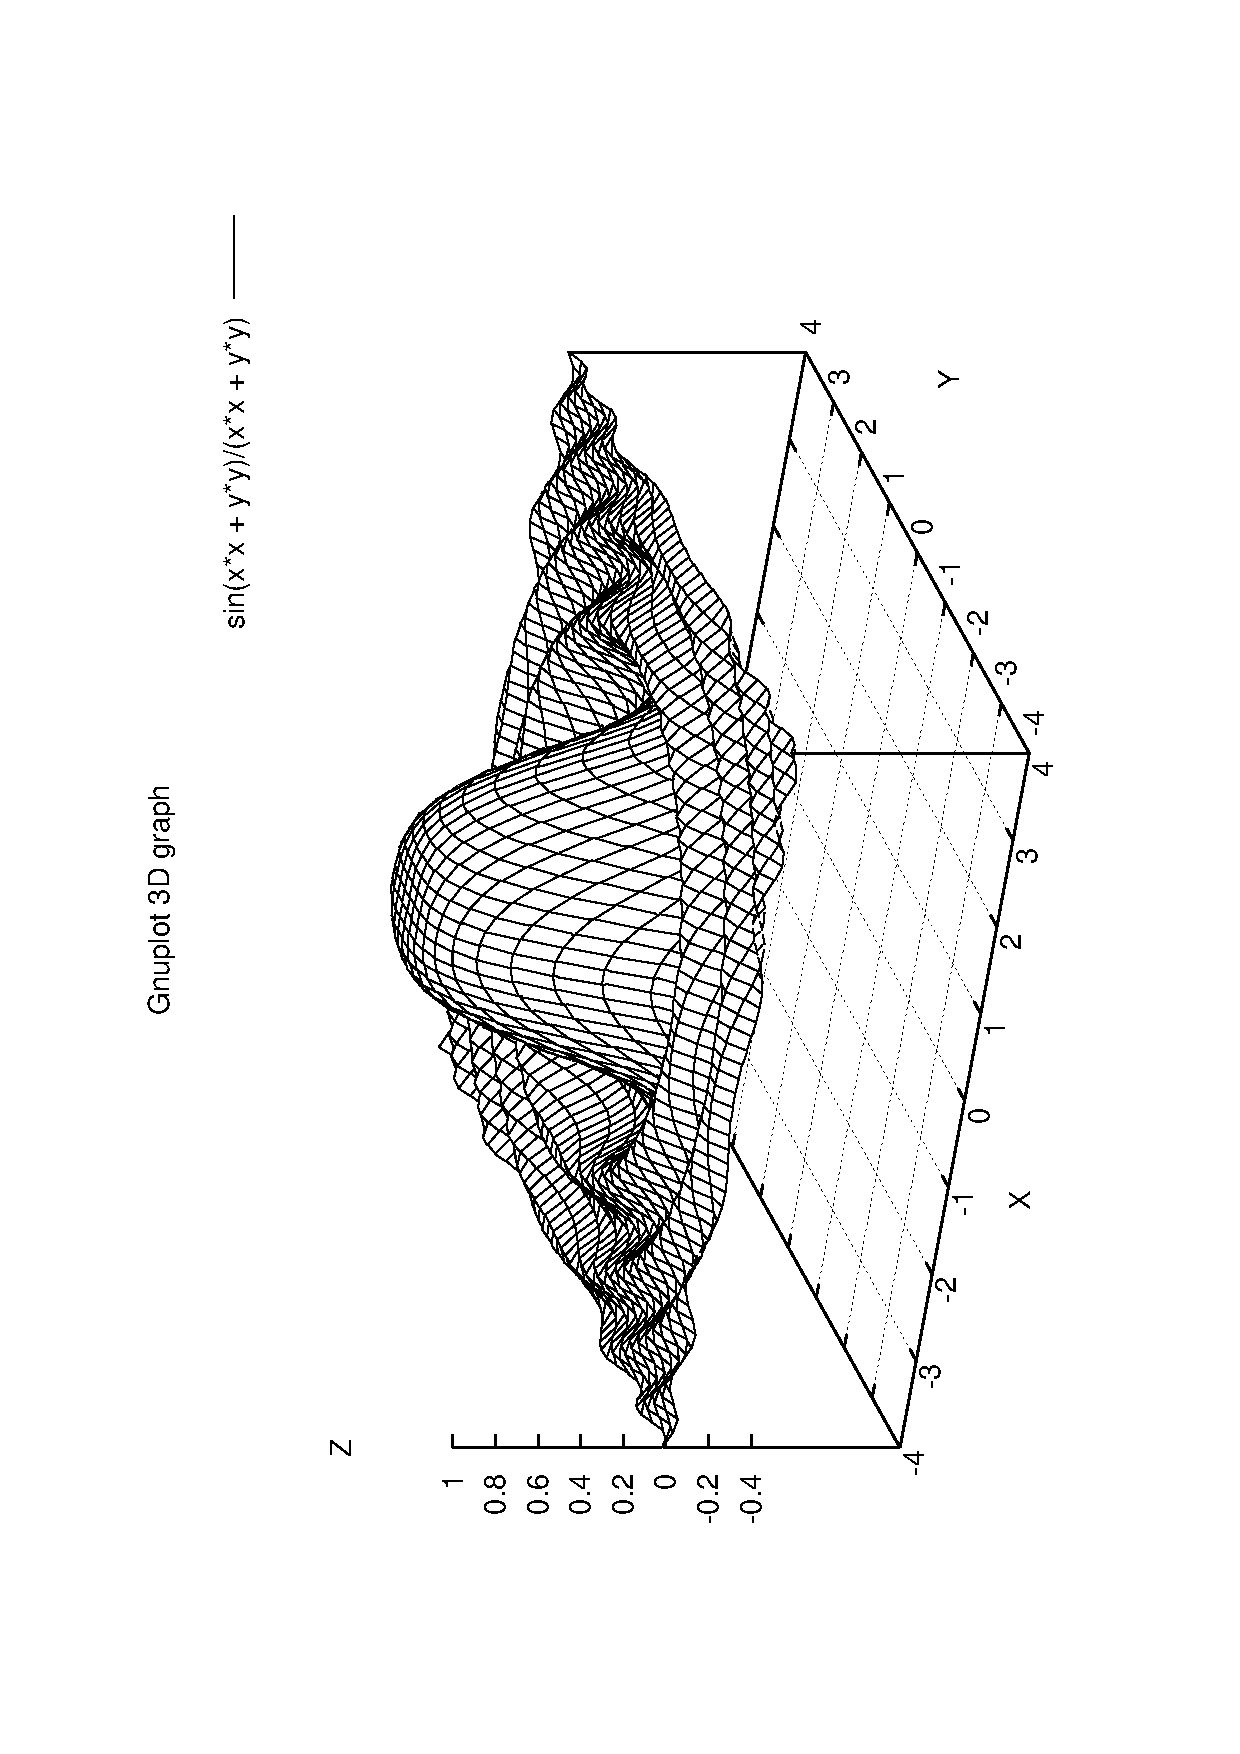
\includegraphics[width=0.6\textwidth, angle=-90]{gnuplot.pdf}}
      \else
        \fbox{\includegraphics[width=0.6\textwidth, angle=-90]{gnuplot.ps}}
      \fi
    \caption{Un grafico fatto con Gnuplot.}
    \label{fig:gnuplot}
    \end{center}
  \end{minipage}
\end{figure}

Componendo un file con \app{latex} e poi \app{dvips}, si possono
includere solo file in formato \file{EPS}; invece, \app{pdflatex}
pu\`o includere file JPG, PNG e ovviamente PDF, il che lo rende
preferibile per la maggior parte degli utenti.

Esistono numerosi programmi per convertire file grafici come
\file{.jpg}, \file{.gif}, \file{.png} ecc. in \file{.eps} e/o
\file{.pdf}; ad esempio, ImageMagik (\url{http://www.imagemagik.org})
e The GIMP (\url{http://www.gimp.org}). Purtroppo, queste applicazioni
generano dei file \PS{} di grosse dimensioni.

Si ottengono risultati migliori con programmi che producono un file
\PS{} compatto tramite la tecnica del ``wrapping'', innestando cio\`e
il file grafico in un file \PS{}. Si raccomandano \app{jpeg2ps}, 
\url{http://www.pdflib.com/jpeg2ps/index.html}, o \app{bmeps},\\ 
\href{http://www.ctan.org/tex-archive/support/bmeps}{CTAN://support/bmeps}.
Il primo dei due \`e spesso il modo migliore per trattare i file
\file{.jpg}, mentre il secondo riesce a gestire pi\`u formati.

Se si vule far s\`\i{} che uno stesso sorgente si possa convertire sia
in PDF che in PS, si devono includere questi comandi:

\begin{Verbatim}[fontsize=\small]
\usepackage{ifpdf}
...
% includi le opzioni giuste
\ifpdf % pdf
  \usepackage[pdftex]{graphicx}
  \pdfcompresslevel=9
\else  % postscript
  \usepackage{graphicx}
\fi
...
% includi il file grafico corretto
\ifpdf % pdf
  \includegraphics{file.png}
\else  % postscript
  \includegraphics{file.eps}
\fi
\end{Verbatim}

\begin{warn}

  Se ci sono pi\`u di 18 figure successive senza del testo
  inframmezzato, si ottiene l'errore \LaTeX{} ``Too many unprocessed
  floats'' (troppi float non ancora gestiti). Il modo pi\`u rapido di
  risolvere il problema \`e scrivere il comando \cmd{clearpage} dopo
  tre o quattro figure.

\end{warn}

% -----

\subsubsection{Testo che scorre intorno alle figure}

\`E possibile ottenere un layout analogo a quello di un giornale o
rivista, col testo che scorre intorno alle figure, tramite il
pacchetto \package{wrapfig}:

\begin{example}
Se incontrate questo tizio,
dategli dei soldi.
\begin{wrapfigure}[4]{l}[5pt]{2cm}
{\Huge
 \texttt{=8-)}
}
\end{wrapfigure}
Magari non capite il perch\'e,
ma vi assicuro che i vostri soldi
finiranno in buone mani.
Ripeto, se incontrate questo tipo,
dategli dei soldi: lui sa come
farne buon uso. Mi raccomando!
\end{example}

I parametri sono:
\begin{inparaenum}[a)]
  \item il numero di linee da fare scorrere intorno alla figura;
  \item il posizionamento della figura (come in \ltx{htbp});
  \item l'\emph{overhang}, cio\`e di quanto deve ``sporgere'' il testo;
  \item la larghezza della figura.
\end{inparaenum}

% -----

% INSERT/SHAPES

\subsection{\entry{Inserisci}{Figura}}

\LaTeX{} fornisce un ambiente \env{picture} entro il quale si possono
usare comandi come \cmd{circle}, \cmd{oval} e molti altri. Ritengo che
tracciare figure senza un ambiente grafico sia un po' troppo
difficile, per non dire poi delle limitazioni intrinseche di
\env{picture}. \`E molto meglio usare un paio di magnifici programmi,
liberi e gratuiti: il programma di grafica vettoriale Inkscape,
\url{https://inkscape.org/}, e Pstoedit, \url{http://www.pstoedit.net/}.

Fate partire Inkscape e disegnate utilizzando i suoi strumenti. Per
inserire del testo composto da \LaTeX, selezionate la voce
\menu{Estensioni/Render/Formula LaTeX...}, inserire il testo come
mostrato in fig.~\ref{fig:ink1}, quindi fare clic su Applica.

\begin{figure}[htbp]
  \centering
  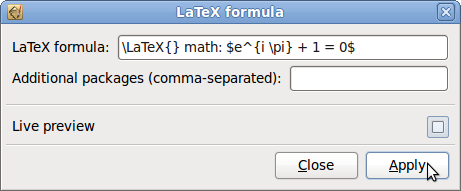
\includegraphics[width=0.6\textwidth]{inkscape-tb.png}
  \caption{Come inserire una formula \LaTeX.}
  \label{fig:ink1}
\end{figure}

Il testo composto da \LaTeX{} verr\`a incluso come oggetto grafico,
che si potr\`a modificare a piacimento. La figura risultante si pu\`o
esportare in diversi formati supportati da \LaTeX, come PDF, PNG e
molti altri. Ulteriori informazioni:
\url{http://www.ctan.org/tex-archive/info/svg-inkscape}.

\begin{figure}[htbp]
  \centering
  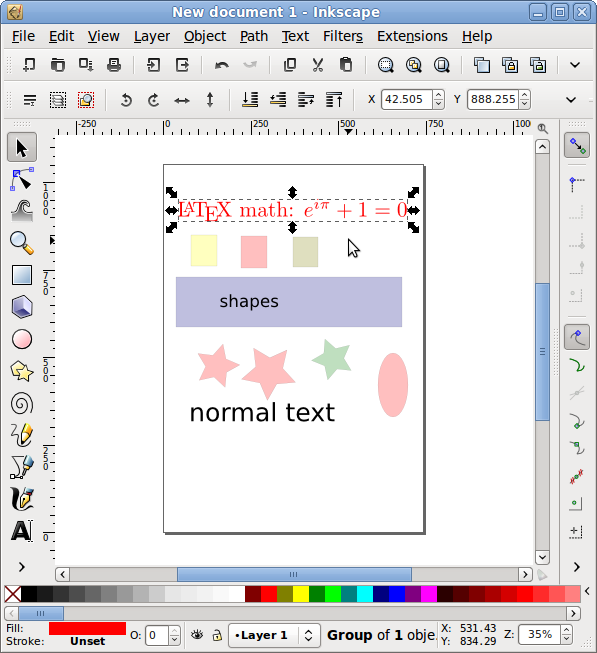
\includegraphics[width=0.6\textwidth]{inkscape.png}
  \caption{Un oggetto \LaTeX{} pu\`o essere modificato.}
  \label{fig:ink2}
\end{figure}

Altri programmi che consentono di creare grafica compatibile con
\LaTeX{} sono i seguenti:

\begin{itemize}
  
  \item \package{pgf}, Portable Graphic Format, \`e un pacchetto
  \TeX{} per generare grafici:\\
  \url{http://sourceforge.net/projects/pgf/}
  
  \item \package{GLE}, Graphics Layout Engine, \`e un linguaggio di
  scripting grafico per creare grafico, diagrammi, figure e
  diapositive di aspetto professionale:\\
  \url{www.gle-graphics.org}
  
  \item Asymptote \`e un linguaggio di grafica vettoriale che fornisce
  un ambiente basato su coordinate per i disegni tecnici:\\
  \url{http://asymptote.sourceforge.net/}
  
  \item ePiX serve per creare figure matematicamente accurate:
  \url{http://mathcs.holycross.edu/~ahwang/current/ePiX.html};
  
  \item \package{pstricks} \`e un insieme di macro per includere
  figure \PS{} in \LaTeX:
  \url{http://tug.org/PSTricks/main.cgi/}
  
\end{itemize}

Questi programmi/pacchetti consentono di creare sofisticate figure in
\LaTeX. Altri programmi sono disponibili in rete; cercate nel web
``LaTeX vector graphics''.

sono disponibili molti altri tipi di `figure'. Per farvi venire
l'acquolina in bocca, visitate la pagina del \TeX{} Showcase,
\url{http://www.tug.org/texshowcase/}.

% -----

% INSERT/LINE

\subsection{\entry{Inserisci}{Righello}}

Si possono tracciare linee di lunghezza e larghezza arbitrarie con
\cmd{rule}:

\begin{example}
Questo \`e un righello
a tutta pagina:\\
\rule{\linewidth}{1pt}
questo invece \`e pi\`u
corto e spesso:\\
\rule{2cm}{2mm}
\end{example}

Un righello pu\`o anche essere composto da punti (\cmd{dotfill});
questo tipo di righello si usa spesso per collegare elementi:

\begin{example}
Prezzo totale \dotfill \euro~10
\end{example}

% -----

% INSERT/HYPERLINK

\subsection{\entry{Inserisci}{Hyperlink}}
\label{sec:hyperlink}

Il pacchetto \package{hyperref} consente di scrivere URL e altri
riferimenti esterni al documento. Usato insieme a \app{dvipdf} o
\app{pdflatex}, \package{hyperref} consente di creare file \file{.pdf}
navigabili! Ad esempio, questa guida contiene questa dichiarazione:

\begin{Verbatim}[fontsize=\small]
\usepackage[colorlinks,
            urlcolor=blue,
	    filecolor=magenta,
	    linkcolor=darkred,
	    hyperfootnotes=false]{hyperref}
\end{Verbatim}

Vediamo un esempio:

\begin{example}
Il sito principale del \hypertarget{ctan}{CTAN}
\`e \url{http://www.ctan.org}, ovvero
\href{http://www.ctan.org}{CTAN://}.

Ascoltate questo
\href{run:midifile.mid}{file MIDI}.

Fare clic \hyperlink{ctan}{qui}
per tornare su.
\end{example}

Come si pu\`o notare, il comando \cmd{url} stampa il suo argomento
utilizzando un font monospaziato. Per usare lo stesso font del testo,
si inserisce il comando:

\begin{Verbatim}
\urlstyle{same}
\end{Verbatim}

dopo la dichiarazione \cmd{hyperref}.

I comandi \cmd{hypertarget} e \cmd{hyperlink} consentono di creare
link interni al documento, proprio come in HTML; \cmd{href} crea link a
URL o file esterni. Si noti il parametro \ltx{run:} si possono
lanciare applicazioni esterne come player multimediali, programmi per
l'ufficio; qualunque cosa. Questa funzionalit\`a viene supportata dai
lettori PDF Adobe Reader, Okular ed Evince.

In ambiente GNU/Linux, e probabilmente anche in altre varianti \unix,
bisogna configurare il lettore PDF per fare in modo che lanci
l'applicazione appropriata quando si fa clic sul relativo link.
Bisogna inserire queste linee nel vostro file \file{.mailcap} o
\file{/etc/mailcap}:

\begin{verbatim}
audio/midi;/usr/bin/timidity %s
audio/*; xmms %s
video/*; xine -pfhq %s
\end{verbatim}

Riferirsi alla documentazione di \package{hyperref} per ulteriori
possibilit\`a.

% -----

% INSERT/COMMENT

\subsection{\entry{Inserisci}{Commento}}

Si fa semplicemente inserendo il carattere \car{\%} prima di ogni
linea, oppure tramite il pacchetto \package{comment} che fornisce
l'omonimo ambiente.

% -----

% FORMAT

\section{Il menu \menu{Formato}}

Principalmente, il formato di un documento viene impostato tramite
appositi parametri in \cmd{document\-class}: grandezza predefinita dei
font (10, 11 o 12pt), formato carta (\ltx{a4paper}, \ltx{a5paper},
\ltx{b5paper}, \ltx{letterpaper}, \ltx{legalpaper},
\ltx{executivepaper}), orientamento della pagina (\ltx{portrait},
\ltx{landscape}). Ad esempio,

\begin{Verbatim}[fontsize=\small]
\documentclass[a5paper,landscape,12pt]{article}
\end{Verbatim}

Si possono specificare altri valori per la grandezza dei font; si veda
alla Sezione~\ref{sec:extsizes}.

% -----

% FORMAT/LINE SPACING

\subsection{\entry{Formato}{Interlinea}}

Il pacchetto \package{setspace} fornisce gli ambienti
\env{singlespace}, \env{onehalfspace} e \env{double\-space}. Inoltre,
il comando \cmd{spacing}\cmdparm{\{fattore\}} (disponibile anche come
ambiente) consente di impostare la spaziatura desiderata:

\begin{example}
\begin{spacing}{2.5}
Queste due linee \\
sono troppo distanziate!
\end{spacing}
\begin{spacing}{1}
Mentre invece queste due linee\\
sono spaziate in modo normale.
\end{spacing}
\end{example}

Se si vuole impostare l'interlinea per tutto il documento, si deve
usare nel preambolo il comando \cmd{linespread\{fattore\}}. Il valore
predefinito di \ltx{factor} \`e 1; valori pi\`u grandi danno un
interlinea maggiore. 1.6 corrisponde all'incirca all'interlinea
doppia.

% -----

% FORMAT/CHARACTER

\subsection{\entry{Formato}{Carattere}}

Gli attributi standard dei caratteri sono elencati alla
Tabella~\ref{tab:properties}, le dimensioni alla
Tabella~\ref{tab:font_sizes}. Si noti che le dimensioni dipendono
dalla dimensione di default impostata in \ltx{docu\-ment\-class} (10,
11 o 12 pt); si veda la Tabella~\ref{tab:font_sizes2}.

\begin{table}[htbp]
\begin{center}
\begin{tabular}{lll} \hline
\textbf{Attributo} & \textbf{Come ambiente} & \textbf{Esempio} \\
\hline
\cmd{textnormal} & \verb|textnormal| & testo normale \\
\cmd{textrm} & \verb|rmfamily| & \textrm{romano} \\
\cmd{textit} & \verb|itshape| & \textit{corsivo} \\
\cmd{emph} & n/a & \emph{corsivo (enfasi)} \\
\cmd{textmd} & \verb|mdseries| & \textmd{normale (default)} \\
\cmd{textbf} & \verb|bfseries| & \textbf{grassetto} \\
\cmd{textup} & \verb|upshape| & \textup{upright (default)} \\
\cmd{textsl} & \verb|slshape| & \textsl{inclinato} \\
\cmd{textsf} & \verb|sffamily| & \textsf{sans serif} \\
\cmd{textsc} & \verb|scshape| & \textsc{maiuscoletto} \\
\cmd{texttt} & \verb|ttfamily| & \texttt{macchina da scrivere} \\
\cmd{underline} & \verb|underline| & \underline{sottolineato} \\
\cmd{textsuperscript} & n/a & testo in \textsuperscript{apice} \\
\cmd{mathrm} & n/a & $\mathrm{x^n + y^n \neq z^n \forall n \neq 2}$ \\
\cmd{mathbf} & n/a & $\mathbf{x^n + y^n \neq z^n \forall n \neq 2}$ \\
\cmd{mathsf} & n/a & $\mathsf{x^n + y^n \neq z^n \forall n \neq 2}$ \\
\cmd{mathtt} & n/a & $\mathtt{x^n + y^n \neq z^n \forall n \neq 2}$ \\
\cmd{mathit} & n/a & $\mathit{x^n + y^n \neq z^n \forall n \neq 2}$ \\
\cmd{mathnormal} & n/a & $\mathnormal{x^n + y^n \neq z^n \forall n \neq 2}$ \\
\cmd{mathcal} & n/a & $\mathcal{x^n + y^n \neq z^n \forall n \neq 2}$ \\
\hline
\end{tabular}
\caption{Attributi dei caratteri.}
\label{tab:properties}
\end{center}
\end{table}

\`E importante capire la differenza tra testo in corsivo
(\cmd{textit}) e testo in enfasi (\cmd{emph}). \textit{Ad esempio,
questa frase \`e scritta in corsivo, e \emph{queste parole} sono
enfatizzate in upright}. Come si pu\`o vedere, \cmd{emph} \`e un
comando di tipo \emph{logico} piuttosto che tipografico.

Inoltre, va ricordato che il testo in pedice si usa solo in modalit\`a
matematica. Per usarlo in modalit\`a testo normale, si fa:

\begin{example}
questo testo \`e in
$_{\mbox{\footnotesize{pedice}}}$
\end{example}

\begin{table}[ht]
\begin{center}
\begin{tabular}{ll} \hline
\textbf{Dimensione} & \textbf{Esempio} \\
\hline
\verb|tiny| & \tiny{testo di esempio} \\
\verb|scriptsize| & \scriptsize{testo di esempio} \\
\verb|footnotesize| & \footnotesize{testo di esempio} \\
\verb|small| & \small{testo di esempio} \\
\verb|normalsize| & \normalsize{testo di esempio} \\
\verb|large| & \large{testo di esempio} \\
\verb|Large| & \Large{testo di esempio} \\
\verb|LARGE| & \LARGE{testo di esempio} \\
\verb|huge| & \huge{testo di esempio} \\
\verb|Huge| & \Huge{testo di esempio} \\
\hline
\end{tabular}
\caption{Dimensione relativa dei font}
\label{tab:font_sizes}
\end{center}
\end{table}

\begin{table}[ht]
\begin{center}
  \begin{tabular}{llll}
  \hline
  Dimensione & 10pt & 11pt & 12pt \\
  \hline
  \ltx{tiny} & 5 & 6 & 6 \\
  \ltx{scriptsize} & 7 & 8 & 8 \\
  \ltx{footnotesize} & 8 & 9 & 10 \\
  \ltx{small} & 9 & 10 & 10.95 \\
  \ltx{normalsize} & 10 & 10.95 & 12 \\
  \ltx{large} & 12 & 12 & 14.4 \\
  \ltx{Large} & 14.4 & 14.4 & 17.28 \\
  \ltx{LARGE} & 17.2 & 17.28 & 20.74 \\
  \ltx{huge} & 20.7 & 20.74 & 24.88 \\
  \ltx{Huge} & 24.8 & 24.88 &  24.88 \\
  \hline
  \end{tabular}
  \caption{Dimensione in punti dei font}
  \label{tab:font_sizes2}
\end{center}
\end{table}

% -----

\subsubsection{Apice e pedice in formule chimiche}

Molte formule chimiche si possono scrivere in modalit\`a matematica,
utilizzando \verb|^| e \verb|_| per ottenere apici e pedici. Il
pacchetto \env{mhchem} formisce un comando che \`e pi\`u semplice da
usare. Le cifre sono stampate in pedice di default, in apice se
precedute da \verb|^|; le formule devono essere incluse in un comando
\cmd{ce}:

\begin{example}
\ce{H2O + CO2 -> H2CO3}\\
\ce{CaCO3 -> Ca^2+ + CO3^2-}\\
\ce{CO3^2- + H2CO3 -> 2 HCO3^-}\\
\ce{CaCO3 + H2CO3 -> Ca^2+ + 2HCO3^-}
\end{example}

% -----

\subsubsection{Testo sottolineato}

Di fatto, lo stile \uline{underline} non si usa pi\`u. La
sottolineatura viene considerata una vecchia eredit\`a delle macchine
da scrivere, e inoltre non ha un bell'aspetto. Se lo si vuole usare
comunque, il pacchetto \package{ulem} mette e disposizione alcuni
stili:

\begin{example}
\uline{importante}
\uuline{urgente}
\uwave{barca}
\sout{sbagliato}
\xout{cancellato}
\end{example}

Attenzione: \package{ulem} ridefinisce il comando \cmd{emph}
(sottolineatura anzich\'e testo enfatizzato). Per fare in modo che
\cmd{emph} mantenga il suo scopo, si deve usare questa dichiarazione:

\begin{verbatim}
\usepackage[normalem]{ulem}
\end{verbatim}


% -----

% FORMAT/CHARACTER SIZE

\subsubsection{\entry{Carattere}{Dimensione}}
\label{sec:extsizes}

Se le dimensioni di default dei font non fossero abbastanza per le
proprie esigenze, si usa il pacchetto \package{extsizes}: fornisce
versioni ``estese'' delle classi di documento standard, con dimensioni
dei font nell'intervallo 8--12, 14, 17 e 20 pt.

Supponiamo di voler scrivere un documento di classe \ltx{article} con
un font a 17 pt. Si deve usare questo preambolo:

\begin{Verbatim}[fontsize=\small]
\documentclass[17pt]{extarticle}
\end{Verbatim}

Un altro modo per ottenere font grandi \`e tramite il pacchetto
\package{type1cm}, che fornisce comandi come questo:

\begin{Verbatim}[fontsize=\small]
\fontsize{72pt}{72pt}\selectfont
Vietato fumare
\end{Verbatim}

(L'esempio qui sopra \`e troppo grande per stare in questa
pagina{\ldots})

I parametri sono la grandezza del font e la baseline. Un altro
approccio \`e il seguente:

\begin{example}
\resizebox{!}{1cm}{alto 1 cm}
\end{example}

\lettrine{L'}{inizio} di un paragrafo pu\`o essere evidenziato
utilizzando il package \package{lettrine}, che fornisce il comando
\cmd{lettrine}, pienamente personalizzabile. Questo paragrafo usa la
definizione di default:

\begin{verbatim}
\lettrine{L'}{inizio} di un paragrafo pu\`o...
\end{verbatim}

% -----

% FORMAT/FONT

\subsubsection{\entry{Carattere}{Font}}

\LaTeX{} utilizza i font Computer Modern, generati dal sottosistema
\MF. Questo approccio garantisce la portabilit\`a e fornisce ottimi
risultati. Molti utenti sono per\`o abituati ad altri font: Times,
Helvetica, Sans Serif{\ldots}

Fortunatamente, \LaTeX{} pu\`o usare i font \PS. Si pu\`o provare ad
utilizzare uno di questi pacchetti: \package{avant},
\package{avangar}, \package{bookman}, \package{chancery},
\package{charter}, \package{courier}, \package{helvet},
\package{helvetic}, \package{ncntrsbk}, \package{newcent},
\package{palatcm}, \package{palatino}, \package{pifont},
\package{times}, \package{utopia}, \package{zapfchan}; ad esempio,
inserendo la dichiara\-zio\-ne \cmd{usepackage\{times\}}. L'unica
avvertenza riguarda la modalit\`a matematica, per la quale i migliori
risultati si hanno con i font Computer Modern; font alternativi
rendono le formule meno eleganti.

I pacchetti sopra elencati impostano il font per l'intero documento.
Se si vuole usare un font \PS{} solo per una parte del testo, si deve
specificare l'insieme di caratteri come nell'esempio che segue. Gli
insiemi di caratteri pi\`u comuni sono elencati alla
Tabella~\ref{tab:font_families}. 

\begin{warn}

  Attenzione: su alcuni sistemi cert font potrebbero non essere
  disponibili!

\end{warn}

\begin{example}
Questo \`e il font
Computer Modern Roman,
{\fontfamily{phv}\selectfont
questo invece \`e Helvetica!}
\end{example}

\begin{table}
\begin{center}
  \begin{tabular}{ll}
  \hline
  \textmd{Family} & \textmd{Name}\\
  \hline
  \ltx{cmr} & Computer Modern Roman\\
  \ltx{cmss} &
  {\fontfamily{cmss}\selectfont Computer Modern Sans Serif}\\
  \ltx{cmtt} &
  {\fontfamily{cmtt}\selectfont Computer Modern Typewriter}\\
  \ltx{pag} &
  {\fontfamily{pag}\selectfont Avantgarde}\\
  \ltx{pbk} &
  {\fontfamily{pbk}\selectfont Bookman}\\
  \ltx{phv} &
  {\fontfamily{phv}\selectfont Helvetica}\\
  \ltx{pnc} &
  {\fontfamily{pnc}\selectfont New Century Schoolbook}\\
  \ltx{ppl} &
  {\fontfamily{ppl}\selectfont Palatino}\\
  \ltx{ptm} &
  {\fontfamily{ptm}\selectfont Times}\\
  \ltx{pcr} &
  {\fontfamily{pcr}\selectfont Courier}\\
  \hline
  \end{tabular}
  \caption{Insiemi di caratteri.}
  \label{tab:font_families}
\end{center}
\end{table}

% \medskip

Un altro metodo ancora \`e la sostituzione di un font \MF{} con uno
\PS; ad esempio, usare Avantgarde ad ogni occorrenza di Computer
Modern Sans Serif. Si fa in questo modo:

\begin{itemize}

  \item \cmd{rmdefault} (roman)
  \item \cmd{sfdefault} (sans serif)
  \item \cmd{ttdefault} (typewriter)
  \item \cmd{bfdefault} (boldface)
  \item \cmd{mddefault} (medium)
  \item \cmd{itdefault} (italics)
  \item \cmd{sldefault} (slanted)
  \item \cmd{scdefault} (small caps)
  \item \cmd{updefault} (upright)

\end{itemize}

\begin{Verbatim}[fontsize=\small]
 % Avantgarde sostituisce sans serif
\renewcommand{\sfdefault}{pag}
\end{Verbatim}

% -----

% FORMAT/COLOUR

\subsubsection{\entry{Carattere}{Colore}}
\label{sec:charcol}

Si possono usare colori nel testo tramite il pacchetto \package{color}
e appositi comandi. I colori predefiniti sono \ltx{black},
\ltx{white}, \ltx{red}, \ltx{green}, \ltx{blue}, \ltx{cyan},
\ltx{magenta}, e \ltx{yellow}, cio\`e nero, bianco, rosso, verde, blu,
azzurro, magenta e giallo. Si possono anche definire dei colori
personalizzati.

\begin{example}
\textcolor{red}{Questo \`e rosso.}\\
\color{blue}
Questo testo \`e blu!\\
Anche questo. Cambiamo colore.\\
\definecolor{mygreen}
{rgb}{0.1,1,0.1}
\color{mygreen}
Questo \`e un bel verde chiaro!\\
\color{black}
\colorbox{cyan}{Un box azzurro}\\
\fcolorbox{blue}{green}
{Un box azzurro contornato di blu}
\end{example}

Inoltre, il comando \cmd{pagecolor} serve per impostare il colore
dell'intera pagina.

% -----

% FORMAT/PARAGRAPH

\subsection{\entry{Formato}{Paragrafo}}

Si ricorda che cosa si intende per ``paragrafo'' in \LaTeX: una parte
di testo delimitata da \car{\bs\bs} oppure seguita da una linea vuota.

Gli \emph{ambienti} (environment) sono il modo principale per
specificare le propriet\`a di un paragrafo, come l'allineamento o il
font. \`E un po' come selezionare il testo con il mouse per poi
scegliere da un menu le propriet\`a desiderate. Un altro modo \`e
racchiudere il testo tra parentesi graffe.

Gli ambienti hanno questa forma:

\begin{Verbatim}[fontsize=\small]
\begin{environment}
...qui va il testo...
\end{environment}
\end{Verbatim}

Ad esempio, per centrare un paragrafo si pu\`o usare l'ambiente
\env{center}:

\begin{example}
\begin{center}
questo testo \`e centrato
\end{center}
\end{example}

Gli ambienti standard sono elencati in Tabella~\ref{tab:environments}.
Nelle prossime sezioni, si mostrer\`a quali usare e come.

\begin{table}[p]
\begin{center}
\begin{tabular}{ll} \hline
\textbf{Environment} & \textbf{Scopo} \\
\hline
\ltx{abstract} & riassunto\\
\ltx{array} & array di formule\\
\ltx{center} & linee centrate\\
\ltx{description} & elenchi con etichetta \\
\ltx{displaymath} & formule matematiche\\
\ltx{document} & inizia un documento\\
\ltx{enumerate} & elenchi numerati\\
\ltx{eqnarray} & sequenza di equazioni allineate\\
\ltx{equation} & mostra un'equazione\\
\ltx{figure} & figura mobile\\
\ltx{flushleft} & testo allineato a sinistra\\
\ltx{flushright} & testo allineato a destra\\
\ltx{itemize} & elenchi puntati\\
\ltx{letter} & lettere\\
\ltx{list} & elenco generico\\
\ltx{math} & formule nel paragrafo\\
\ltx{minipage} & mini pagina\\
\ltx{picture} & immagine con testo e figure geometriche\\
\ltx{quotation} & citazione con testo indentato\\
\ltx{quote} & citazione senza indentazione\\
\ltx{tabbing} & tabulazioni\\
\ltx{table} & tabelle mobili\\
\ltx{tabular} & testo allineato in colonne\\
\ltx{thebibliography} & bibliografia\\
\ltx{theorem} & teoremi, lemmi ecc.\\
\ltx{titlepage} & prime pagine personalizzate\\
\ltx{verbatim} & testo letterale\\
\ltx{verse} & poesie e simili\\
\hline
\end{tabular}
\caption{Ambienti standard di \LaTeX}
\label{tab:environments}
\end{center}
\end{table}

% -----

% FORMAT/PARAGRAPH HORIZONTAL ALIGNMENT

\subsubsection{\entry{Paragrafo}{Allineamento orizzontale}}

Il testo viene allineato ai margini, per default. Per avere il testo
allineato solo a sinistra, a destra o centrato, si usano gli
ambienti \env{flushleft}, \env{flushright} e \env{center}. I
comandi \cmd{raggedright}, \cmd{raggedleft} e \cmd{centering} sono
equivalenti agli ambienti, ma non iniziano un nuovo paragrafo.

% -----

% FORMAT/PARAGRAPH VERTICAL ALIGNMENT

\subsubsection{\entry{Paragrafo}{Allineamento verticale}}

Una delle differenze che confonde maggiormente gli utenti di word
processor \`e il modo in cui i paragrafi vengono separati in \LaTeX.
\emph{Una o pi\`u linee vuote vengono considerate equivalenti a una
sola linea vuota; lo stesso vale per gli spazi}. In altre parole, non
si pu\`o ottenere pi\`u spazio tra paragrafi inserendo linee vuote.
Per spaziarli, si usano i comandi \cmd{smallskip}, \cmd{medskip} e
\cmd{bigskip} per ottenere una spaziatura piccola, media o grande.

Se serve pi\`u spazio, si pu\`o usare il comando
\cmd{vskip}\{\textit{parametro}\} come in questo esempio:

\begin{example}
Questi paragrafi saranno
separati di 1,3 cm:\\
\vskip 1.3cm
c'\`e uno spazio di 1,3 cm
sopra di me.
\end{example}

Va notato che \cmd{vskip} funziona solo tra paragrafi. Come si fa
allora per iniziare una pagina dopo un margine aggiuntivo di (ad es.)
1,3 cm? Si deve usare il comando \cmd{null}, che fa da ``segnaposto''
nel testo:

\begin{example}
\null
\vskip 1.3 cm
Linea che inizia dopo 1,3 cm.
\end{example}

Infine, il comando \cmd{vfill} si usa per aggiungere un ``riempimento
verticale'', ad esempio per inserire linee vuote tra paragrafi in modo
che il secondo si trovi esattamente a fine pagina:

% \begin{example} will not work here
% \medskip

\begin{minipage}[c]{0.49\textwidth}
  \begin{Verbatim}[fontsize=\small]
  Questo testo appare all'inizio
  della pagina{\ldots}
  \vfill
  {\ldots}e questo invece alla fine.
  \end{Verbatim}
\end{minipage}
\begin{boxedminipage}[c]{0.49\textwidth}
  Questo testo appare all'inizio
  della pagina{\ldots}
  \vskip 1.3 cm
  {\ldots}e questo invece alla fine.
\end{boxedminipage}

% -----

% FORMAT/PARAGRAPH MARGINS

\subsubsection{\entry{Paragrafo}{Margini}}

Di solito, si impostano i margini per l'intero documento come abbiamo
visto alla Sezione~\ref{sec:pagesetup}. Ridefinirli temporaneamente
per una parte del testo non funziona: per reimpostare i margini per
uno o pi\`u paragrafi, si deve creare un nuovo ambiente come questo:

\begin{Verbatim}[fontsize=\small]
\newenvironment{margini}[2]
{ 
  \begin{list}{} {
    \setlength{\leftmargin}{#1}
    \setlength{\rightmargin}{#2}
  } \item }
{\end{list}}
\end{Verbatim}

Il nuovo ambiente si usa cos\`\i{}:

\begin{example}
Come si pu\`o vedere, questo
paragrafo ha i margini
predefiniti.
\begin{margini}{0.5cm}{1cm}
Ma attenzione: li abbiamo
cambiati per questo paragrafo!
\end{margini}
\end{example}

% -----

% FORMAT/PARAGRAPH INDENTATION

\subsubsection{\entry{Paragrafo}{Rientro}}

Per impostare il rientro di un paragrafo, si modifica il valore del
contatore \cmd{parindent}. In questo esempio, impostiamo il rientro
di 1 cm:

\begin{Verbatim}[fontsize=\small]
\setlength{\parindent}{1cm}
\end{Verbatim}

I comandi \cmd{indent} e \cmd{noindent} consentono o impediscono il
rientro nel paragrafo successivo. Infine, la distanza tra paragrafi si
imposta con il contatore \cmd{parskip}:

\begin{Verbatim}[fontsize=\small]
\setlength{\parskip}{3pt}
\end{Verbatim}

% -----

% FORMAT/BORDER

\subsubsection{\entry{Paragrafo}{Bordi e ombreggiatura}}

Per avere parole o paragrafi circondati da un bordo, si usano il
pacchetto \package{framed} e/o il comando \cmd{parbox}. Nel secondo
caso, \`e anche necessario il pacchetto \package{calc}.

Il metodo pi\`u facile \`e usare \package{framed}:

% \begin{example} will not work here
\bigskip

\begin{minipage}[c]{0.5\textwidth}
  \begin{Verbatim}[fontsize=\small]
  \setlength{\FrameRule}{2pt}
  \setlength{\FrameSep}{5pt}
  \begin{framed}
    questo paragrafo ha il bordo!
  \end{framed}
  \definecolor{shadecolor}{rgb}
  {0.8,0.8,1}
  \begin{shaded}
    questo paragrafo \`e
    ombreggiato, vi piace?
  \end{shaded}
  \end{Verbatim}
\end{minipage}%
\begin{minipage}[c]{0.5\textwidth}
\setlength{\FrameRule}{2pt}
\setlength{\FrameSep}{5pt}
\begin{framed}
  questo paragrafo ha il bordo!
\end{framed}
\definecolor{shadecolor}{rgb}
  {0.8,0.8,1}
  \begin{shaded}
    questo paragrafo \`e
    ombreggiato, vi piace?
  \end{shaded}
\end{minipage}

\bigskip

In modo equivalente, si pu\`o fare con il pacchetto
\package{boxedminipage} e l'omonimo ambiente. Per chi vuole saperne di
pi\`u: i comandi

\begin{Verbatim}[fontsize=\small]
\framebox{
  \begin{minipage}[c]{\linewidth}
  testo da bordare
  \end{minipage}
}
\end{Verbatim}

danno gli stessi risultati dell'ambiente \env{boxedminipage}.

% Questo esempio usa invece \cmd{parbox}:

% \begin{example}
% \noindent
% \fbox{
%   \parbox{\linewidth%
%     -2 \fboxsep -2 \fboxrule}
%   {un altro paragrafo col bordo}
% }
% \end{example}

\cmd{width} imposta la larghezza della minipage uguale a quella del
testo. Si pu\`o ovviamente impostare la larghezza che si preferisce.

Infine, si pu\`o impostare un bordo che si adatti alla larghezza del
testo:

\begin{example}
questa \`e una
\framebox[\width]{parola}
con il bordo.
\end{example}

Si pu\`o variare la larghezza modificando il parametro di
\cmd{framebox}:

\begin{example}
questa \`e un'altra
\framebox[2\width][r]{parola}
con il bordo.
\end{example}

Notare il secondo parametro opzionale, che permette di indicare un
allineamento (a destra nell'esempio).

% -----

% FORMAT/COLOUR

\subsubsection{\entry{Paragrafo}{Colore}}

Ora che si ha un bordo, si potr\`a impostare anche un colore di
sfondo:

\begin{example}
\colorbox{yellow}{
  \begin{minipage}
  {0.8\linewidth}
  Questa \`e una minipage
  di colore giallo!
  \end{minipage}
}
\end{example}

A scopo esemplificativo, il colore \`e stato limitato all'80\% della
minipage. Alla Sezione~\ref{sec:charcol} verranno spiegati altri
dettagli sull'uso dei colori.

% -----

% FORMAT/COLUMNS

\subsection{\entry{Formato}{Colonne}}

I comandi \cmd{twocolumn} e \cmd{onecolumn} iniziano una nuova pagina
e impostano il numero di colonne del testo; si possono usare anche
xcome parametri in \cmd{documentclass}. Se ancora non basta, il
pacchetto \package{multicols} fornisce l'omonimo ambiente. Si sarebbe
potuta impostare questa sezione in due colonne con i comandi:

\begin{Verbatim}[fontsize=\small]
\columnseprule=1pt
\begin{multicols}{2}[\subsection{\entry{Formato}{Colonne}}]
I comandi \cmd{twocolumn} e \cmd{onecolumn} ...
\end{multicols}
\end{Verbatim}

Lo spazio tra le colonne si imposta con il parametro \cmd{columnsep},
lo spessore della linea tra le colonne con \cmd{columnseprule}. Il
testo specificato come parametro opzionale tra le parentesi quadre
viene escluso dall'ambiente.

% -----

% TABLE

\section{Il menu \menu{Tabella}}
\label{sec:table}

Le tabelle sono un argomento piuttosto complesso{\ldots} Una tabella
\`e un oggetto mobile (come spiegato alla Sezione~\ref{sec:figure})
che deve essere compreso in una pagina. Normalmente contiene un
ambiente \env{tabular}, ma ci sono altre possibilit\`a. Per default,
una tabella si adatta automaticamente alla larghezza dei suoi
contenuti.

Va sottolineato che l'ambiente \env{table} \`e un oggetto mobile, ma
l'ambiente \env{tabular} non lo \`e. Di questo va tenuto conto se si
vogliono scrivere tabelle ``informali'', cio\`e senza etichetta e
didascalia.

Questo \`e il formato generale di una tabella:

\begin{Verbatim}[fontsize=\footnotesize]
\begin{table}[htbp] % posizione: qui, alto, basso, pagina separata
% \begin{small}     % imposta il font della tabella
\begin{center}      % opzionale
% tabella a 4 colonne; allieneamento a sx, centro, dx, larghezza fissa
\begin{tabular}{|l|c|rp{4cm}|} 
\hline              % linea orizzontale
\textbf{Sinistra} & \textbf{Centro} & \textbf{Destra} & \textbf{4 cm} \\
\hline
riga 1, col 1 & riga 1, col 2 & riga 1, col 3 & riga 1, col 4 \\
\cline{1-2}         % linea orizz. estesa tra le colonne 1-2
riga 2, col 1 & riga 2, col 2 & riga 2, col 3 & riga 2, col 4 \\
\cline{1-2}
\multicolumn{2}{|c|}{esteso tra due colonne} & riga 3, col 3 & 
riga 3, col 4 \\
\cline{1-3}
riga 4, col 1 & riga 4, col 2 & riga 4, col 3 & ~ \hfill destra \\
% force a space with "\ "
riga 5, col 1 & riga 5, col 2 & riga 5, col 3 & sinistra \hfill ~ \\
riga 5, col 1 & riga 5, col 2 & riga 5, col 3 & 
~ \hfill centro \hfill ~ \\
\hline
\end{tabular}
\caption{Una tabella di esempio.}
% le etichette si usano per i riferimenti;
% ad esempio, ``si veda la Tabella~\ref{tab:sampletab}"
\label{tab:sampletab}
\end{center}
% \end{small}
\end{table}
\end{Verbatim}

La tabella~\ref{tab:sampletab} mostra i risultati.

\begin{table}[htbp] % posizione: qui, alto, basso, pagina separata
% \begin{small}     % imposta il font della tabella
\begin{center}      % opzionale
% tabella a 4 colonne; allieneamento a sx, centro, dx, larghezza fissa
\begin{tabular}{|l|c|rp{4cm}|} 
\hline              % linea orizzontale
\textbf{Sinistra} & \textbf{Centro} & \textbf{Destra} & \textbf{4 cm} \\
\hline
riga 1, col 1 & riga 1, col 2 & riga 1, col 3 & riga 1, col 4 \\
\cline{1-2}         % linea orizz. estesa tra le colonne 1-2
riga 2, col 1 & riga 2, col 2 & riga 2, col 3 & riga 2, col 4 \\
\cline{1-2}
\multicolumn{2}{|c|}{esteso tra due colonne} & riga 3, col 3 & 
riga 3, col 4 \\
\cline{1-3}
riga 4, col 1 & riga 4, col 2 & riga 4, col 3 & ~ \hfill destra \\
% force a space with "\ "
riga 5, col 1 & riga 5, col 2 & riga 5, col 3 & sinistra \hfill ~ \\
riga 5, col 1 & riga 5, col 2 & riga 5, col 3 & 
~ \hfill centro \hfill ~ \\
\hline
\end{tabular}
\caption{Una tabella di esempio.}
% le etichette si usano per i riferimenti;
% ad esempio, ``si veda la Tabella~\ref{tab:sampletab}"
\label{tab:sampletab}
\end{center}
% \end{small}
\end{table}

Talvolta, una tabella \`e troppo larga e non rientra nei margini della
pagina. In questo caso, il pacchetto \package{rotating} fornisce
l'ambiente \env{sidewaystable}. Inoltre, \package{rotating} rende
possibile ruotare i contenuti di una cella di un angolo specificato.
Esiste anche il pacchetto \package{tabularx} che consente di
specificare tabelle di larghezza fissa tramite il parametro \ltx{X},
che indica che una colonna pu\`o espandersi a richiesta.

Ecco un esempio:

% \begin{example} will not work here
\bigskip

\begin{minipage}{0.7\textwidth}
  \begin{Verbatim}[fontsize=\small]
  \begin{sidewaystable}
    \begin{tabularx}{7.5cm}{|l|X|X|}
      \hline
      \textbf{normale} & \textbf{inclinato} & 
      \textbf{pi\`u largo} \\
      \hline
      normale & \rotatebox{30}{inclinato!} & 
      pi\`u largo \\
      \hline
    \end{tabularx}
  \end{sidewaystable}
\end{Verbatim}
\end{minipage}%
\begin{minipage}{0.3\textwidth}
% qui imbrogliamo: tabularx non funziona in una minipage,
% quindi carichiamo la figura.
\ifpdf
  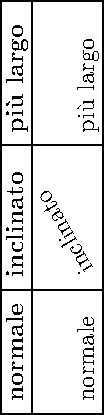
\includegraphics{tbx.pdf}
\else
  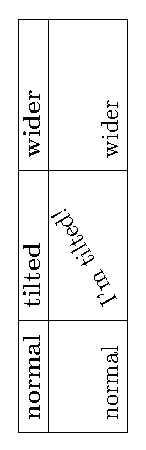
\includegraphics{tbx.epsi}
\fi
\end{minipage}

\bigskip

Si ricorda \note che l'ambiente \env{tabular} standard non pu\`o
estendersi oltre una pagina! Ci sono pacchetti che consentono di
superare questa limitazione: si raccomandano \package{longtable},
\package{supertabular} e \package{xtab}.

Per avere righe o celle colorate, si usa il pacchetto
\package{colortbl}:

\begin{example}
Colore per linea:\\\vskip 2mm
\begin{tabular}{|l|c|r|}
  \hline
  \rowcolor{cyan}
  uno & due & tre\\
  \rowcolor{green}
  uno & due & tre\\
  \rowcolor{yellow}
  uno & due & tre\\
  \hline
\end{tabular}
\end{example}

\begin{example}
Colore per colonna:\\\vskip 2mm
\begin{tabular}
  {|>{\columncolor{cyan}}l|
  >{\color{red}
  \columncolor{green}}c|
  >{\columncolor{yellow}}r|}
  \hline
  uno & due & tre\\
  uno & due & tre\\
  uno & due & tre\\
  \hline
\end{tabular}
\end{example}

Per concludere l'argomento tabella, ecco un suggerimento. Se si 
ritiene che scrivere le tabelle \LaTeX{} sia troppo complicato, si
pu\`o trovare un valido aiuto in OpenOffice Calc e Calc2LaTeX. Il
primo di questi \`e il noto foglio elettronico Open Source, il secondo
\`e una componente aggiuntiva che serve per convertire un insieme di
celle in una tabella \LaTeX. Link: \url{http://www.openoffice.org/}, 
\url{http://calc2latex.sourceforge.net/}.

% -----

\subsection{\entry{Tabella}{Interlinea}}

Una linea della tabella prende l'altezza del testo che contiene. Per
aggiungere dello spazio \emph{prima} di una linea, si pu\`o usare il
trucco di iniziarla con un \ltx{\textbackslash{}rule} di lunghezza 0 e
altezza specificata. Per aggiungere spazio \emph{dopo} la linea, si
usa \ltx{\textbackslash{}\textbackslash{}} seguito da un parametro
opzionale che specifica lo spazio.

Ecco un esempio:

\begin{example}
\begin{tabular}{lll}
uno & due & tre\\
0.3 centimetri & \textbf{dopo} &
questa linea\\[0.3cm]
uno & due & tre\\
uno & due & tre\\
\rule{0pt}{1.2cm}1.2 centimetri &
  \textbf{prima} & di questa linea\\
\end{tabular}
\end{example}

% -----

\subsection{\entry{Tabella}{Larghezza del righello}}

% TO DO: \setlength{\arrayrulewidth}{<width>}

\begin{example}
\begin{tabular}{|lll|}
\hline
\setlength{\arrayrulewidth}{25pt}
uno & due & tre\\
\hline
quattro & cinque & sei\\
%\setlength{\arrayrulewidth}{1pt}
\hline
\end{tabular}
\end{example}

% -----

\subsection{\entry{Tabella}{Allineamento dei numeri}}

Un caso particolare dell'ambiente \env{tabular} \`e quando si vogliono
allineare dei numeri rispetto alle posizioni decimali.

Il modo pi\`u semplice \`e tramite lo specificatore di colonna
\verb-@-, che in pratica serve solo in tabelle che contengano solo
numeri. Il separatore di colonna \ltx{\&} \`e sostituito dal punto
decimale:

\begin{example}
\begin{tabular}{r@{.}l}
 3&14159\\
 1&61803\\
 1&41421\\
 100&00000
\end{tabular}
\end{example}

Come alternativa, si usa il pacchetto \package{dcolumn}, che aggiunge
lo specificatore di colonna \ltx{D}. \ltx{D} ha tre argomenti: il
separatore da usare nel sorgente \LaTeX{} e in output (solitamente lo
stesso, ``.'') e il numero di cifre alla destra dell'indicatore della
posizione decimale. Inoltre, il terzo parametro opzionale pu\`o
indicare il numero di cifre a sinistra e a destra del punto decimale,
separate appunto da un punto. Infine, se il terzo parametro \`e -1, i
numeri della colonna verranno centrati intorno al separatore decimale.

I contenuti della tabella sono stampati in modalit\`a matematica. Per
inserire delle intestazioni, si dovr\`a includere il testo in un
\cmd{mbox}.

% \begin{example} will not work here
\bigskip

\begin{minipage}[c]{0.5\textwidth}
  \begin{Verbatim}[fontsize=\small]
  \begin{tabular}{|D{.}{,}{4.2}|%
  D{.}{.}{5}|D{.}{.}{-1}|}
  \hline
  \mbox{Uno} & \mbox{Due} &
  \mbox{Tre} \\
  10.33 & 10.33 & 10.33 \\
  1000 & 1000 & 1000 \\
  5.1 & 5.1 & 5.1 \\
  3.14 & 3.14159 & 3.14159 \\
  \hline
  \end{tabular}
  \end{Verbatim}
\end{minipage}%
\begin{minipage}[c]{0.5\textwidth}
\begin{tabular}{|D{.}{,}{4.2}|%
D{.}{.}{5}|D{.}{.}{-1}|}
\hline
\mbox{Uno} & \mbox{Due} &
\mbox{Tre} \\
10.33 & 10.33 & 10.33 \\
1000 & 1000 & 1000 \\
5.1 & 5.1 & 5.1 \\
3.14 & 3.14159 & 3.14159 \\
\hline
\end{tabular}
\end{minipage}

% -----

\subsection{Il pacchetto \package{slashbox}}

Questo pacchetto aggiunge il comando \cmd{backslashbox}.

\bigskip

\begin{minipage}[c]{0.5\textwidth}
  \begin{Verbatim}[fontsize=\small]
\begin{tabular}{|l|l|l|}
  \hline
  \backslashbox[2cm]{Lezione}{Data} & 
  Luned\`\i{} & Marted\`\i{} \\
  \hline
  Stratigrafia & aula A & aula A \\
  Chimica & aula B & Lab $\alpha$ \\
  Fisica & aula C & Lab $\beta$ \\
  \hline
\end{tabular}
\end{Verbatim}
\end{minipage}%
\begin{minipage}[c]{0.5\textwidth}
\begin{tabular}{|l|l|l|}
  \hline
  \backslashbox[2cm]{Lezione}{Data} & 
  Luned\`\i{} & Marted\`\i{} \\
  \hline
  Stratigrafia & aula A & aula A \\
  Chimica & aula B & Lab $\alpha$ \\
  Fisica & aula C & Lab $\beta$ \\
  \hline
\end{tabular}
\end{minipage}

% \emph{TODO: mention \cmd{newcolumntype} e \package{floatflt}}

% -----

\subsection{Importare dati in tabelle \LaTeX}

Per molte persone, i file di dati numerici rappresentano il lavoro
quotidiano. Molti file di dati sono semplici file ASCII contenenti
colonne di numeri; altri file solo invece prodotti con fogli
elettronici. Praticamente tutti i fogli elettronici possono esportare
i dati in formato \file{.csv}; i valori sono di solito separati con il
carattere ``;''.

Convertire un file di dati in una tabella \LaTeX{} \`e un lavoro
complesso e noioso. Lo script seguente, per sistemi \unix, svolge
questo lavoro di conversione in automatico; funziona anche per
convertire file \file{.csv}. Richiede il programma \app{awk}.

\begin{Verbatim}[fontsize=\small]  
#!/bin/sh

# dat2tex: converte dati tabellari in un ambiente tabular

if [ $# != 1 ]; then
  echo "Uso: $0 <datafile>"
  exit 1
fi

# e' un file csv?
grep ";" $1 > /dev/null
if [ $? = 0 ]; then
  AWK="awk -F;"
else
  AWK=awk
fi

# forza awk, buon lavoro
$AWK '{if (1 == FNR) { \
        printf "\\begin{tabular}{"; \
        for (i = 1; i <= NF; i++) {printf "l"}; \
        printf "}\n"
      }
      for (i = 1; i < NF; i++) \
        {printf $i" & "} printf $NF" \\\\ \n"} \
      END {printf "\\end{tabular}\n"}' $1

# fine del file dat2tex
\end{Verbatim}

% -----

% TOOLS

\section{Il menu \menu{Strumenti}}

% -----

% TOOLS/MAIL MERGES

\subsection{\entry{Strumenti}{Stampa unione}}

Questa utilissima funzionalit\`a viene implementata dal pacchetto
\package{textmerg}. Si consideri un semlice documento, ad esempio una
lettera, nella quale possono variare il nome, cognome e titolo della
persona cui stiamo scrivendo. Il testo rimanente non cambia.

Si dovranno definire tre \emph{campi}, che rappresentano la parte
variabile del testo: \cmd{Nome}, \cmd{Cognome} e \cmd{Titolo}. I
rispettivi valori verranno letti da un file di testo, \file{dati.dat}.

\begin{Verbatim}[fontsize=\small]
\documentclass{article}
\usepackage{textmerg}
\begin{document}
% dichiariamo i campi variabili:
% \Void serve per linee vuote.
\Fields{\Nome\Cognome\Titolo-\Void}
\Merge{dati.dat}{%
Caro \Titolo{} \Cognome,\\
posso chiamarti \Nome?\\
Cordialmente,\\
\hspace{3cm}Guido\clearpage}
\end{document}
\end{Verbatim}

Il quarto campo, \cmd{Void}, qui in realt\`a non serve ed \`e incluso
solo per esempio. Viene preceduto da un segno meno, il che significa
che nel file di dati questo campo pu\`o essere vuoto. In altre parole,
si vogliono separare i campi con linee vuote.

Questo \`e il file \file{dati.dat}:

\begin{Verbatim}[fontsize=\small]
Guido
Gonzato
Dr.

Francesco
Mulargia
Prof.

Marie
Curie
Mme

\end{Verbatim}

Tutto qui: l'output risultante conterr\`a il testo adattato per
ciascuno dei destinatari, una pagina per ognuno.

% -----

% TOOLS/LABELS

\subsection{\entry{Strumenti}{Etichette}}

Se \`e stato facile realizzare la stampa unione, \`e addirittura
banale stampare delle etichette. Si supponga di voler stampare 20
etichette su di un foglio adesivo che ne contiene 3$\times$8. Si deve
usare il pacchetto \package{labels}; nell'esempio che segue, si
stamperanno 10 etichette normali e 10 col bordo:

\begin{Verbatim}[fontsize=\small]
\documentclass[a4paper,12pt]{article}
\usepackage{labels}
\LabelCols=3      % n. di colonne di etichette
\LabelRows=8      % n. di righe di etichette
\LeftBorder=8mm   % bordi di ciascuna etichetta
\RightBorder=8mm
\TopBorder=5mm
\BottomBorder=5mm
\LabelGridtrue      % mostra una griglia
\numberoflabels=10  % n. di etichetta da stampare per ogni tipo
% il testo dell'etichetta si specifica
% tramite la macro \addresslabel[]{}:
\begin{document}
  \addresslabel[\large] % argomenti opzionali
  {\textbf{Guido Gonzato}, Ph.D.\\
  \textsl{Linux system manager}}
  % etichette col bordo
  \boxedaddresslabel[\fboxsep=4mm\fboxrule=1mm]
  {\textbf{Guido Gonzato}, Ph.D.\\
  \textsl{Linux system manager}}
\end{document}
\end{Verbatim}

% You'll also have to choose the correct paper size e adjust the page
% margins (use \package{geometry}; omitted in this example).

Per realizzare etichette che contengano diversi indirizzi, si pu\`o
usare un file esterno o inserire gli indirizzi nel file principale:

\begin{Verbatim}[fontsize=\small]
\documentclass[a4paper,12pt]{article}
\usepackage{labels}
\LabelCols=3
\LabelRows=8
\LeftBorder=3mm
\RightBorder=3mm
\TopBorder=8mm
\BottomBorder=8mm
\LabelGridtrue
\begin{document}
% usare questo ambiente:
\begin{labels}
  1$^{o}$ nome
  1$^{o}$ indirizzo
  1$^{o}$ citt\`a, CAP

  2$^{o}$ nome
  2$^{o}$ indirizzo
  2$^{o}$ citt\`a, CAP

  3$^{o}$ nome
  3$^{o}$ indirizzo
  3$^{o}$ citt\`a, CAP
\end{labels}
% oppure un file esterno contenente 
% esattamente lo stesso testo:
% \labelfile{addresses.dat}
\end{document}
\end{Verbatim}

Si lascia come esercizio al lettore la combinazione dei pacchetti
\package{textmerg} e \package{labels}!

% -----

% TOOLS/LANGUAGE

\subsection{\entry{Strumenti}{Lingua}}

La lingua predefinita di \LaTeX{} \`e l'inglese, ma ovviamente ne
supporta altre, tra cui l'italiano. Per ``lingua'' si intende la
traduzione automatica di termini come ``Chapter'' o ``Index'' in
``Capitolo'' e ``Indice'', la sillabazione e la possibilit\`a di
inserire direttamente i caratteri accentati (il modo standard \`e
tramite combinazioni di caratteri: \car{\`e} si inserisce con
\ltx{\bs{}`e}.)

Le distribuzioni \LaTeX{} contengono un file chiamato
\file{language.dat} (di solito in
\path{$TEXMF/tex/generic/config/language.dat}) che contiene un elenco
di lingue. Questo file si pu\`o editare per aggiungere la lingua
italiana.

Inoltre, \`e importante il pacchetto \package{babel} che serve per
attivare il supporto per la lingua italiana:

\begin{Verbatim}[fontsize=\small]
\usepackage[italian]{babel}
\end{Verbatim}

\begin{warn}

  \package{babel} pu\`o cambiare il modo in cui alcuni caratteri
  vengono trattati da \LaTeX. Se ci si imbatte in problemi inattesi,
  si dovranno inserire i caratteri problematici tramite la sintassi
  \cmd{charXX}. A me \`e capitato con il carattere \char94.

\end{warn}

Per inserire lettere accentate e in generale i caratteri ASCII non
standard\footnote{in gergo informatico, i ``caratteri ASCII standard''
sono quelli il cui codice \`e compreso tra 32 (spazio) e 126
(tilde).}, si possono usare i pacchetti \package{inputenc} e
\package{fontenc}, specificando l'encoding desiderato. UTF-8 dovrebbe
essere la scelta corretta, e dovr\`a essere impostato anche per il
proprio editor:

\begin{Verbatim}[fontsize=\small]
\usepackage[utf8]{inputenc}
\usepackage[T1]{fontenc}
\end{Verbatim}

Un modo alternativo per non inserire le lettere accentate a mano \`e
quello di configurare l'editor per farlo in automatico. Ad esempio, ho
configurato il mio editor preferito (\app{jed}) in modo che inserisca
\ltx{\bs{}'e} quando batto la lettera \car{\`e}. Ecco che cosa ho
incluso nel mio file \file{.jedrc}:

{\small
\begin{alltt}
define latex_mode_hook ()
\{
  set_abbrev_mode (1);
  if ( () = abbrev_table_p ("LaTeX") )
    use_abbrev_table ("LaTeX");
#ifdef WIN32
  % prevent clash with movement keys
  undefinekey ("\`a\`a", "LaTeX-Mode");
  definekey (" \bs\bs`a", "\`a\`a", "LaTeX-Mode");
#else
  local_setkey (" \bs\bs`a",     "\`a");
#endif
  local_setkey (" \bs\bs'e",     "\'e");
  local_setkey (" \bs\bs`e",     "\`e");
  local_setkey (" \bs\bs`\bs\bs{}i\{\}", "\`\i");
  local_setkey (" \bs\bs`o",     "\`o");
  local_setkey (" \bs\bs`u",     "\`u");
\}
\end{alltt}
}

Si  dovr\`a verificare nella documentazione del proprio editor.

% -----

% TOOLS/HYPHEN

\subsection{\entry{Strumenti}{Sillabazione}}

Per quanto \LaTeX{} in genere faccia un buon lavoro di sillabazione,
talvolta pu\`o rendersi necessario un intervento manuale. La
sillabazione si indica inserendo \car{\bs-} nel punto dove si vuole 
che la parola sia divisa. Un altro modo \`e specificando delle regole
di sillabazione per un elenco di parole:

\begin{Verbatim}[fontsize=\small]
\hyphenation{geo-fi-si-ca geo-lo-gia Terra}
\end{Verbatim}

Questa dichiarazione indica che la parola ``Terra'' non deve essere
divisa. Un altro modo per impedire che una parola sia sillabata \`e
quello di racchiuderla in un \cmd{mbox}:

\begin{Verbatim}[fontsize=\small]
Sono un masochista, quindi non voglio sillabare
la parola \mbox{internazionalizzazione}.
\end{Verbatim}

% -----

% TOOLS/SPELL CHECK

\subsection{\entry{Strumenti}{Ortografia}}

\LaTeX{} non si occupa di ortografia. Il controllo ortografico si fa
tramite strumenti esterni come \app{ispell}, \app{aspell} o altri
ancora. In ambiente \unix, si usa \app{ispell} in questo modo:

\begin{Verbatim}[fontsize=\small]
shell> ispell -t -d italiano documento.tex
\end{Verbatim}

Lo switch \ltx{-t} indica a \app{ispell} di ignorare i comandi \TeX{}
e \LaTeX. Lo switch \ltx{-d} serve per specificare il dizionario
italiano.

% -----

% HELP

\section{Il menu \menu{Aiuto}}

Ci sono molti modi di ottenere aiuto con \LaTeX, anche online. Il sito
principale da cui iniziare \`e la pagina apposita del CTAN,
\url{http://www.ctan.org/tex-archive/info/}.

\begin{itemize}

  \item \cmdline{info latex} o \cmdline{info latex2e} (sistemi \unix)
  fornisce una guida concisa ma completa sui comandi e i concetti;
  
  \item \url{http://www.ctan.org/tex-archive/info/LatexHelpBook/} \`e
  un sistema di aiuto per \LaTeX, integrato con Windows.
    
  \item da non scordare il gruppo di discussione 
  \url{http://groups.google.com/group/comp.text.tex/topics}: \`e
  un'importantissima fonte di aiuto da parte di altri utenti.
  
\end{itemize}

Molte distribuzioni GNU/Linux forniscono \app{TeXLive}, che \`e
probabilmente il sistema \LaTeX{} pi\`u completo. Con esso viene
fornita molta documentazione; sul mio sistema Ubuntu, si trova in 
\path{/usr/share/doc/texlive-doc/}.

% -----

\section{Fine}

Questo documento \`e copyleft \textcopyright{} Guido Gonzato,
2001--2015, e distribuito sotto licenza GNU Free Documentation
Licence. Spero che vi possa risultare utile. Per ogni commento o
suggerimento, contattatemi pure.

\newpage

% -----

\appendix

\section{Modelli di documento}
\label{ap:templates}

Un modello per la classe \ltx{article} \`e stato presentato alla
Sezione~\ref{sec:filenew}. Altri modelli sono mostrati nelle figure
seguenti.

% -----

% LIBRO

\begin{figure}[htbp]
\begin{Verbatim}[fontsize=\small]
\documentclass[twoside,11pt]{book}
\begin{document}
\frontmatter
\begin{titlepage}
\title{Il mio libro}
\end{titlepage}
\author{Guido Gonzato}
\maketitle
\tableofcontents
\mainmatter
\part{L'inizio}
\chapter{Introduzione}
\section{Iniziamo}
Il libro inizia qui.
\part{Fine}
\backmatter
Grazie per aver letto il mio libro.
\end{document}
\end{Verbatim}
\caption{Modello di documento di classe \ltx{book}.}
\end{figure}

% -----

% REPORT

\begin{figure}[htbp]
\begin{Verbatim}[fontsize=\small]
\documentclass[twoside,12pt]{report}
% tabelle e figure alla fine:
\usepackage{endfloat}
\begin{document}
\title{Relazione finale}
\author{Guido Gonzato}
\date{Verona, \today}
\maketitle
\begin{abstract}
Questa \`e la relazione finale.
\end{abstract}
\tableofcontents
\listoftables
\listoffigures
\part{Prima parte}
\chapter{Inizio}
\section{Introduzione}
La relazione inizia qui.
\end{document}
\end{Verbatim}
\caption{Modello di documento di classe \ltx{report}.}
\end{figure}

% -----

% LETTERA

\begin{figure}[htbp]
\begin{Verbatim}[fontsize=\small]
\documentclass[12pt]{letter}
\begin{document}
\address{Il mio indirizzo}
\signature{Guido}
\begin{letter}{indirizzo del destinatario}
\opening{Caro Tizio,}
Grazie tante per la birra.
...
\closing{Spero di rivederti presto,}
\ps{P.S. Salutami tua sorella!}
\encl{Le foto di mio figlio}
\end{letter}
\end{document}
\end{Verbatim}
\caption{Modello di documento di classe \ltx{letter}.}
\end{figure}

% -----

% AVVISO

\begin{figure}[htbp]
\begin{Verbatim}[fontsize=\small]
\documentclass[a4paper]{article}
\usepackage{type1cm}
\usepackage{times}
\usepackage{color}
\usepackage{rotating}
\pagestyle{empty}
\begin{document}
\begin{sidewaysfigure}
  \fontsize{2.5cm}{2.5cm}\selectfont
  \centerline{\textcolor{blue}{\textbf{Per piacere:}}}
  \vskip 1cm
  \fontsize{4cm}{3cm}\selectfont
  \centerline{\textcolor{red}{NON FUMATE}}
  \centerline{\textcolor{red}{IN QUESTA}}
  \centerline{\textcolor{red}{STANZA!}}
  \vskip 1cm
  \fontsize{2cm}{2cm}\selectfont
  \centerline{\textcolor{magenta}{Se lo fate,}}
  \centerline{\textcolor{magenta}{verrete \emph{disossati!}}}
\end{sidewaysfigure}
\end{document}
\end{Verbatim}
\caption{Come scrivere un volantino.}
\end{figure}

% -----

% POSTER

\begin{figure}[htbp]
\begin{Verbatim}[fontsize=\small]
\documentclass{article}
\usepackage[absolute,showboxes]{textpos}
\usepackage{color}
\usepackage{framed}
\usepackage{graphicx}
\setlength{\TPHorizModule}{10mm} % unita' di misura: modulo
\setlength{\TPVertModule}{\TPHorizModule}
\setlength{\TPboxrulesize}{1pt}  % spessore linea
% l'angolo in alto a sinistra e' l'origine
\textblockorigin{0mm}{0mm}

\begin{document}
\setlength{\parindent}{0pt}
\definecolor{shadecolor}{rgb}{0.9,1,1}
\begin{textblock}{5}(0,0)
% questo blocco e' largo 5 moduli;
% l'altezza e' automatica
\begin{center}
  \begin{minipage}[c]{0.8 \linewidth}
  \begin{shaded}
  Questo blocco ha l'angolo in alto a sx all'``origine''
  della pagina, impostata a (0mm,0mm). Il margine interno
  e l'ombreggiatura sono creati dagli ambienti
  \texttt{minipage} e \texttt{shaded}.
  \end{shaded}
  \end{minipage}
\end{center}
\end{textblock}
\begin{textblock}{6}(10,1)
  \includegraphics[width=6cm,angle=-90]{gnuplot.ps}
  Questa figura sta a (10,1). Notare che ruotandola
  di -90 gradi fa uscire il margine.
\end{textblock}
\begin{textblock}{5}[0.5,0.5](2.5,8)
Questo blocco sta a (2.5,8); ma poich\'e si \`e specificato
l'argomento opzionale [0.5,0.5], \`e il centro del blocco
a trovarsi in quella posizione, invece dell'angolo superiore
sinistro.
\end{textblock}
\begin{textblock}{3,4}(6,4)
Le dimensioni di questo blocco sono 3$\times$4 cm.
L'origine \`e (6,4) nella pagina. Notare che il testo
supera il margine in alcuni punti; per impedirlo, usare
l'ambiente \env{minipage}.
\end{textblock}
\end{document}
\end{Verbatim}
\caption{Come scrivere un poster.}
\label{fig:poster}
\end{figure}

% -----

% Fine

\end{document}
